\documentclass[twoside]{book}

% Packages required by doxygen
\usepackage{fixltx2e}
\usepackage{calc}
\usepackage{doxygen}
\usepackage[export]{adjustbox} % also loads graphicx
\usepackage{graphicx}
\usepackage[utf8]{inputenc}
\usepackage{makeidx}
\usepackage{multicol}
\usepackage{multirow}
\PassOptionsToPackage{warn}{textcomp}
\usepackage{textcomp}
\usepackage[nointegrals]{wasysym}
\usepackage[table]{xcolor}

% Font selection
\usepackage[T1]{fontenc}
\usepackage[scaled=.90]{helvet}
\usepackage{courier}
\usepackage{amssymb}
\usepackage{sectsty}
\renewcommand{\familydefault}{\sfdefault}
\allsectionsfont{%
  \fontseries{bc}\selectfont%
  \color{darkgray}%
}
\renewcommand{\DoxyLabelFont}{%
  \fontseries{bc}\selectfont%
  \color{darkgray}%
}
\newcommand{\+}{\discretionary{\mbox{\scriptsize$\hookleftarrow$}}{}{}}

% Page & text layout
\usepackage{geometry}
\geometry{%
  a4paper,%
  top=2.5cm,%
  bottom=2.5cm,%
  left=2.5cm,%
  right=2.5cm%
}
\tolerance=750
\hfuzz=15pt
\hbadness=750
\setlength{\emergencystretch}{15pt}
\setlength{\parindent}{0cm}
\setlength{\parskip}{3ex plus 2ex minus 2ex}
\makeatletter
\renewcommand{\paragraph}{%
  \@startsection{paragraph}{4}{0ex}{-1.0ex}{1.0ex}{%
    \normalfont\normalsize\bfseries\SS@parafont%
  }%
}
\renewcommand{\subparagraph}{%
  \@startsection{subparagraph}{5}{0ex}{-1.0ex}{1.0ex}{%
    \normalfont\normalsize\bfseries\SS@subparafont%
  }%
}
\makeatother

% Headers & footers
\usepackage{fancyhdr}
\pagestyle{fancyplain}
\fancyhead[LE]{\fancyplain{}{\bfseries\thepage}}
\fancyhead[CE]{\fancyplain{}{}}
\fancyhead[RE]{\fancyplain{}{\bfseries\leftmark}}
\fancyhead[LO]{\fancyplain{}{\bfseries\rightmark}}
\fancyhead[CO]{\fancyplain{}{}}
\fancyhead[RO]{\fancyplain{}{\bfseries\thepage}}
\fancyfoot[LE]{\fancyplain{}{}}
\fancyfoot[CE]{\fancyplain{}{}}
\fancyfoot[RE]{\fancyplain{}{\bfseries\scriptsize Generated by Doxygen }}
\fancyfoot[LO]{\fancyplain{}{\bfseries\scriptsize Generated by Doxygen }}
\fancyfoot[CO]{\fancyplain{}{}}
\fancyfoot[RO]{\fancyplain{}{}}
\renewcommand{\footrulewidth}{0.4pt}
\renewcommand{\chaptermark}[1]{%
  \markboth{#1}{}%
}
\renewcommand{\sectionmark}[1]{%
  \markright{\thesection\ #1}%
}

% Indices & bibliography
\usepackage{natbib}
\usepackage[titles]{tocloft}
\setcounter{tocdepth}{3}
\setcounter{secnumdepth}{5}
\makeindex

% Hyperlinks (required, but should be loaded last)
\usepackage{ifpdf}
\ifpdf
  \usepackage[pdftex,pagebackref=true]{hyperref}
\else
  \usepackage[ps2pdf,pagebackref=true]{hyperref}
\fi
\hypersetup{%
  colorlinks=true,%
  linkcolor=blue,%
  citecolor=blue,%
  unicode%
}

% Custom commands
\newcommand{\clearemptydoublepage}{%
  \newpage{\pagestyle{empty}\cleardoublepage}%
}

\usepackage{caption}
\captionsetup{labelsep=space,justification=centering,font={bf},singlelinecheck=off,skip=4pt,position=top}

%===== C O N T E N T S =====

\begin{document}

% Titlepage & ToC
\hypersetup{pageanchor=false,
             bookmarksnumbered=true,
             pdfencoding=unicode
            }
\pagenumbering{alph}
\begin{titlepage}
\vspace*{7cm}
\begin{center}%
{\Large E\+E\+CE 435L Project }\\
\vspace*{1cm}
{\large Generated by Doxygen 1.8.13}\\
\end{center}
\end{titlepage}
\clearemptydoublepage
\pagenumbering{roman}
\tableofcontents
\clearemptydoublepage
\pagenumbering{arabic}
\hypersetup{pageanchor=true}

%--- Begin generated contents ---
\chapter{Hierarchical Index}
\section{Class Hierarchy}
This inheritance list is sorted roughly, but not completely, alphabetically\+:\begin{DoxyCompactList}
\item Q\+Graphics\+Pixmap\+Item\begin{DoxyCompactList}
\item \contentsline{section}{game2}{\pageref{classgame2}}{}
\item \contentsline{section}{left\+\_\+disks}{\pageref{classleft__disks}}{}
\item \contentsline{section}{leftbutton}{\pageref{classleftbutton}}{}
\item \contentsline{section}{mid\+\_\+disks}{\pageref{classmid__disks}}{}
\item \contentsline{section}{midbutton}{\pageref{classmidbutton}}{}
\item \contentsline{section}{right\+\_\+disks}{\pageref{classright__disks}}{}
\item \contentsline{section}{rightbutton}{\pageref{classrightbutton}}{}
\end{DoxyCompactList}
\item Q\+Graphics\+Scene\begin{DoxyCompactList}
\item \contentsline{section}{game2}{\pageref{classgame2}}{}
\end{DoxyCompactList}
\item Q\+Object\begin{DoxyCompactList}
\item \contentsline{section}{left\+\_\+disks}{\pageref{classleft__disks}}{}
\item \contentsline{section}{leftbutton}{\pageref{classleftbutton}}{}
\item \contentsline{section}{mid\+\_\+disks}{\pageref{classmid__disks}}{}
\item \contentsline{section}{midbutton}{\pageref{classmidbutton}}{}
\item \contentsline{section}{right\+\_\+disks}{\pageref{classright__disks}}{}
\item \contentsline{section}{rightbutton}{\pageref{classrightbutton}}{}
\end{DoxyCompactList}
\item Q\+Widget\begin{DoxyCompactList}
\item \contentsline{section}{battleship}{\pageref{classbattleship}}{}
\item \contentsline{section}{Battleship\+\_\+\+Main\+\_\+\+Menu}{\pageref{classBattleship__Main__Menu}}{}
\item \contentsline{section}{game2\+\_\+main\+\_\+menu}{\pageref{classgame2__main__menu}}{}
\item \contentsline{section}{historypanel}{\pageref{classhistorypanel}}{}
\item \contentsline{section}{login\+Panel}{\pageref{classloginPanel}}{}
\item \contentsline{section}{lose\+\_\+screen}{\pageref{classlose__screen}}{}
\item \contentsline{section}{mainpanel}{\pageref{classmainpanel}}{}
\item \contentsline{section}{question\+\_\+tab}{\pageref{classquestion__tab}}{}
\item \contentsline{section}{signup\+\_\+form}{\pageref{classsignup__form}}{}
\item \contentsline{section}{victory\+\_\+screen}{\pageref{classvictory__screen}}{}
\item \contentsline{section}{welcome\+\_\+screen}{\pageref{classwelcome__screen}}{}
\end{DoxyCompactList}
\end{DoxyCompactList}

\chapter{Class Index}
\section{Class List}
Here are the classes, structs, unions and interfaces with brief descriptions\+:\begin{DoxyCompactList}
\item\contentsline{section}{\hyperlink{classbattleship}{battleship} }{\pageref{classbattleship}}{}
\item\contentsline{section}{\hyperlink{classBattleship__Main__Menu}{Battleship\+\_\+\+Main\+\_\+\+Menu} }{\pageref{classBattleship__Main__Menu}}{}
\item\contentsline{section}{\hyperlink{classgame2}{game2} }{\pageref{classgame2}}{}
\item\contentsline{section}{\hyperlink{classgame2__main__menu}{game2\+\_\+main\+\_\+menu} }{\pageref{classgame2__main__menu}}{}
\item\contentsline{section}{\hyperlink{classhistorypanel}{historypanel} }{\pageref{classhistorypanel}}{}
\item\contentsline{section}{\hyperlink{classleft__disks}{left\+\_\+disks} }{\pageref{classleft__disks}}{}
\item\contentsline{section}{\hyperlink{classleftbutton}{leftbutton} }{\pageref{classleftbutton}}{}
\item\contentsline{section}{\hyperlink{classloginPanel}{login\+Panel} }{\pageref{classloginPanel}}{}
\item\contentsline{section}{\hyperlink{classlose__screen}{lose\+\_\+screen} }{\pageref{classlose__screen}}{}
\item\contentsline{section}{\hyperlink{classmainpanel}{mainpanel} }{\pageref{classmainpanel}}{}
\item\contentsline{section}{\hyperlink{classmid__disks}{mid\+\_\+disks} }{\pageref{classmid__disks}}{}
\item\contentsline{section}{\hyperlink{classmidbutton}{midbutton} }{\pageref{classmidbutton}}{}
\item\contentsline{section}{\hyperlink{classquestion__tab}{question\+\_\+tab} }{\pageref{classquestion__tab}}{}
\item\contentsline{section}{\hyperlink{classright__disks}{right\+\_\+disks} }{\pageref{classright__disks}}{}
\item\contentsline{section}{\hyperlink{classrightbutton}{rightbutton} }{\pageref{classrightbutton}}{}
\item\contentsline{section}{\hyperlink{classsignup__form}{signup\+\_\+form} }{\pageref{classsignup__form}}{}
\item\contentsline{section}{\hyperlink{classvictory__screen}{victory\+\_\+screen} }{\pageref{classvictory__screen}}{}
\item\contentsline{section}{\hyperlink{classwelcome__screen}{welcome\+\_\+screen} }{\pageref{classwelcome__screen}}{}
\end{DoxyCompactList}

\chapter{File Index}
\section{File List}
Here is a list of all documented files with brief descriptions\+:\begin{DoxyCompactList}
\item\contentsline{section}{\hyperlink{battleship_8cpp}{battleship.\+cpp} \\*Battleship }{\pageref{battleship_8cpp}}{}
\item\contentsline{section}{\hyperlink{battleship_8h}{battleship.\+h} \\*Battleship class }{\pageref{battleship_8h}}{}
\item\contentsline{section}{\hyperlink{battleship__main__menu_8cpp}{battleship\+\_\+main\+\_\+menu.\+cpp} \\*Battleship main menu }{\pageref{battleship__main__menu_8cpp}}{}
\item\contentsline{section}{\hyperlink{battleship__main__menu_8h}{battleship\+\_\+main\+\_\+menu.\+h} \\*Battleship main menu class }{\pageref{battleship__main__menu_8h}}{}
\item\contentsline{section}{\hyperlink{extern__vars_8h}{extern\+\_\+vars.\+h} \\*Extern\+\_\+vars class }{\pageref{extern__vars_8h}}{}
\item\contentsline{section}{\hyperlink{game2_8cpp}{game2.\+cpp} \\*Game2 }{\pageref{game2_8cpp}}{}
\item\contentsline{section}{\hyperlink{game2_8h}{game2.\+h} \\*Game2 class }{\pageref{game2_8h}}{}
\item\contentsline{section}{\hyperlink{game2__main__menu_8cpp}{game2\+\_\+main\+\_\+menu.\+cpp} \\*Game2 main menu }{\pageref{game2__main__menu_8cpp}}{}
\item\contentsline{section}{\hyperlink{game2__main__menu_8h}{game2\+\_\+main\+\_\+menu.\+h} \\*Game2 main meenu class }{\pageref{game2__main__menu_8h}}{}
\item\contentsline{section}{\hyperlink{historypanel_8cpp}{historypanel.\+cpp} \\*User game history implementation }{\pageref{historypanel_8cpp}}{}
\item\contentsline{section}{\hyperlink{historypanel_8h}{historypanel.\+h} \\*User game history }{\pageref{historypanel_8h}}{}
\item\contentsline{section}{\hyperlink{left__disks_8cpp}{left\+\_\+disks.\+cpp} \\*Left discs }{\pageref{left__disks_8cpp}}{}
\item\contentsline{section}{\hyperlink{left__disks_8h}{left\+\_\+disks.\+h} \\*Left discs class }{\pageref{left__disks_8h}}{}
\item\contentsline{section}{\hyperlink{leftbutton_8cpp}{leftbutton.\+cpp} \\*Leftbutton }{\pageref{leftbutton_8cpp}}{}
\item\contentsline{section}{\hyperlink{leftbutton_8h}{leftbutton.\+h} \\*Leftbutton class }{\pageref{leftbutton_8h}}{}
\item\contentsline{section}{\hyperlink{loginpanel_8cpp}{loginpanel.\+cpp} \\*Implementation of login menu }{\pageref{loginpanel_8cpp}}{}
\item\contentsline{section}{\hyperlink{loginpanel_8h}{loginpanel.\+h} \\*Loginpanel header class }{\pageref{loginpanel_8h}}{}
\item\contentsline{section}{\hyperlink{lose__screen_8cpp}{lose\+\_\+screen.\+cpp} \\*Lose screen implementation of lose screen class }{\pageref{lose__screen_8cpp}}{}
\item\contentsline{section}{\hyperlink{lose__screen_8h}{lose\+\_\+screen.\+h} \\*Lose\+\_\+screen class }{\pageref{lose__screen_8h}}{}
\item\contentsline{section}{\hyperlink{mainpanel_8cpp}{mainpanel.\+cpp} \\*Mainpanel }{\pageref{mainpanel_8cpp}}{}
\item\contentsline{section}{\hyperlink{mainpanel_8h}{mainpanel.\+h} \\*Mainpanel header class }{\pageref{mainpanel_8h}}{}
\item\contentsline{section}{\hyperlink{mid__disks_8cpp}{mid\+\_\+disks.\+cpp} \\*Mid discs }{\pageref{mid__disks_8cpp}}{}
\item\contentsline{section}{\hyperlink{mid__disks_8h}{mid\+\_\+disks.\+h} \\*Mid discs class }{\pageref{mid__disks_8h}}{}
\item\contentsline{section}{\hyperlink{midbutton_8cpp}{midbutton.\+cpp} \\*Midbutton }{\pageref{midbutton_8cpp}}{}
\item\contentsline{section}{\hyperlink{midbutton_8h}{midbutton.\+h} \\*Midbutton class }{\pageref{midbutton_8h}}{}
\item\contentsline{section}{{\bfseries question\+\_\+tab.\+h} }{\pageref{question__tab_8h}}{}
\item\contentsline{section}{\hyperlink{right__disks_8h}{right\+\_\+disks.\+h} \\*Right discs class }{\pageref{right__disks_8h}}{}
\item\contentsline{section}{\hyperlink{rightbutton_8h}{rightbutton.\+h} \\*Rightbutton class }{\pageref{rightbutton_8h}}{}
\item\contentsline{section}{\hyperlink{signup__form_8cpp}{signup\+\_\+form.\+cpp} \\*Signup\+\_\+form }{\pageref{signup__form_8cpp}}{}
\item\contentsline{section}{\hyperlink{signup__form_8h}{signup\+\_\+form.\+h} \\*For registering new users }{\pageref{signup__form_8h}}{}
\item\contentsline{section}{\hyperlink{victory__screen_8cpp}{victory\+\_\+screen.\+cpp} \\*Victory screen }{\pageref{victory__screen_8cpp}}{}
\item\contentsline{section}{\hyperlink{victory__screen_8h}{victory\+\_\+screen.\+h} \\*Victory screen class }{\pageref{victory__screen_8h}}{}
\item\contentsline{section}{\hyperlink{welcome__screen_8cpp}{welcome\+\_\+screen.\+cpp} \\*Screen that shows when user logins in }{\pageref{welcome__screen_8cpp}}{}
\item\contentsline{section}{\hyperlink{welcome__screen_8h}{welcome\+\_\+screen.\+h} \\*Header file for \hyperlink{welcome__screen_8cpp}{welcome\+\_\+screen.\+cpp} }{\pageref{welcome__screen_8h}}{}
\end{DoxyCompactList}

\chapter{Class Documentation}
\hypertarget{classbattleship}{}\section{battleship Class Reference}
\label{classbattleship}\index{battleship@{battleship}}


Inheritance diagram for battleship\+:\nopagebreak
\begin{figure}[H]
\begin{center}
\leavevmode
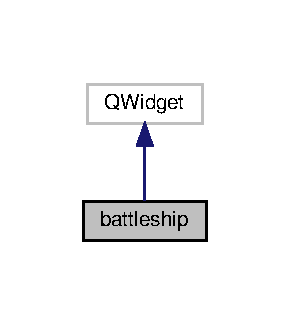
\includegraphics[width=139pt]{classbattleship__inherit__graph}
\end{center}
\end{figure}


Collaboration diagram for battleship\+:\nopagebreak
\begin{figure}[H]
\begin{center}
\leavevmode
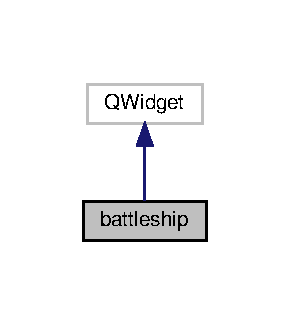
\includegraphics[width=139pt]{classbattleship__coll__graph}
\end{center}
\end{figure}
\subsection*{Public Slots}
\begin{DoxyCompactItemize}
\item 
bool \hyperlink{classbattleship_a0744ad364092e726f52bdaac336581e5}{open\+\_\+question\+\_\+tab} ()
\begin{DoxyCompactList}\small\item\em Function that opens a question tab when a player clicks on a button. \end{DoxyCompactList}\item 
void \hyperlink{classbattleship_afd1d4e449ff0b266871eca956b406b2b}{show\+Ship00} ()
\begin{DoxyCompactList}\small\item\em Function that checks if a ship is under a pushbutton. \end{DoxyCompactList}\item 
\mbox{\Hypertarget{classbattleship_ad6379760759a77a0b479983b08068138}\label{classbattleship_ad6379760759a77a0b479983b08068138}} 
void {\bfseries show\+Ship01} ()
\item 
\mbox{\Hypertarget{classbattleship_ac5e8d56e60d0cd00c23b2391de838416}\label{classbattleship_ac5e8d56e60d0cd00c23b2391de838416}} 
void {\bfseries show\+Ship02} ()
\item 
\mbox{\Hypertarget{classbattleship_a1bd31ba45a22552797d03914fabdfa5b}\label{classbattleship_a1bd31ba45a22552797d03914fabdfa5b}} 
void {\bfseries show\+Ship03} ()
\item 
\mbox{\Hypertarget{classbattleship_a21c04d344578bc5ccf50ec8bb6143cc5}\label{classbattleship_a21c04d344578bc5ccf50ec8bb6143cc5}} 
void {\bfseries show\+Ship10} ()
\item 
\mbox{\Hypertarget{classbattleship_a072ca835236dc8cbae004e6295d55eba}\label{classbattleship_a072ca835236dc8cbae004e6295d55eba}} 
void {\bfseries show\+Ship11} ()
\item 
\mbox{\Hypertarget{classbattleship_ade3e18ff71103bed1baf78fd551460f2}\label{classbattleship_ade3e18ff71103bed1baf78fd551460f2}} 
void {\bfseries show\+Ship12} ()
\item 
\mbox{\Hypertarget{classbattleship_ac22320ed94718a56d6c03593a26ae0e1}\label{classbattleship_ac22320ed94718a56d6c03593a26ae0e1}} 
void {\bfseries show\+Ship13} ()
\item 
\mbox{\Hypertarget{classbattleship_a77ea25213dad52f754ca640225c5bafa}\label{classbattleship_a77ea25213dad52f754ca640225c5bafa}} 
void {\bfseries show\+Ship20} ()
\item 
\mbox{\Hypertarget{classbattleship_a7a8bdac9d5fdab5b9c2f644cbb907f23}\label{classbattleship_a7a8bdac9d5fdab5b9c2f644cbb907f23}} 
void {\bfseries show\+Ship21} ()
\item 
\mbox{\Hypertarget{classbattleship_a9c6154eb4707452f5198e45d8c8dbd8e}\label{classbattleship_a9c6154eb4707452f5198e45d8c8dbd8e}} 
void {\bfseries show\+Ship22} ()
\item 
\mbox{\Hypertarget{classbattleship_a13de6528e0911afc18408d2b97f9762c}\label{classbattleship_a13de6528e0911afc18408d2b97f9762c}} 
void {\bfseries show\+Ship23} ()
\item 
\mbox{\Hypertarget{classbattleship_a9ba8dd0642ad8399c773ca9e18b14769}\label{classbattleship_a9ba8dd0642ad8399c773ca9e18b14769}} 
void {\bfseries show\+Ship30} ()
\item 
\mbox{\Hypertarget{classbattleship_a5773f762c98d1d175b0f22551e478586}\label{classbattleship_a5773f762c98d1d175b0f22551e478586}} 
void {\bfseries show\+Ship31} ()
\item 
\mbox{\Hypertarget{classbattleship_aef3cfb89e65bc1b668f72e5c0164fb2c}\label{classbattleship_aef3cfb89e65bc1b668f72e5c0164fb2c}} 
void {\bfseries show\+Ship32} ()
\item 
\mbox{\Hypertarget{classbattleship_afaa4f0016271f47183cdd9f48230c9db}\label{classbattleship_afaa4f0016271f47183cdd9f48230c9db}} 
void {\bfseries show\+Ship33} ()
\item 
void \hyperlink{classbattleship_ad6e6acff47dd594732ad1606b62a9dbc}{update\+Timer} ()
\begin{DoxyCompactList}\small\item\em Function for updating the timer. \end{DoxyCompactList}\end{DoxyCompactItemize}
\subsection*{Public Member Functions}
\begin{DoxyCompactItemize}
\item 
\hyperlink{classbattleship_ac40d202657fb7498a3ed6c6c625a3ca6}{battleship} (Q\+Widget $\ast$parent=nullptr)
\item 
void \hyperlink{classbattleship_a3e06e47874fec7fb9cc1fd23589d6f72}{check\+Counters} ()
\begin{DoxyCompactList}\small\item\em Function that checks if a pushbutton has been clicked. \end{DoxyCompactList}\item 
void \hyperlink{classbattleship_afddb8a1aca235146e2cc11e2b3c54d01}{get\+User} (Q\+String)
\begin{DoxyCompactList}\small\item\em Function that gets the username. \end{DoxyCompactList}\item 
void \hyperlink{classbattleship_a72fd3ca8ec081b72c888ffb8b5f95153}{save\+Score} (Q\+String player, int correct, int incorrect)
\begin{DoxyCompactList}\small\item\em Function that saves the user\textquotesingle{}s score. \end{DoxyCompactList}\end{DoxyCompactItemize}
\subsection*{Public Attributes}
\begin{DoxyCompactItemize}
\item 
\mbox{\Hypertarget{classbattleship_a696e12a77797e57b9cb42157ff1bcf6e}\label{classbattleship_a696e12a77797e57b9cb42157ff1bcf6e}} 
Q\+Time $\ast$ \hyperlink{classbattleship_a696e12a77797e57b9cb42157ff1bcf6e}{timer}
\begin{DoxyCompactList}\small\item\em timer for game duration \end{DoxyCompactList}\item 
\mbox{\Hypertarget{classbattleship_a30c0ca88edbc62d56adb987b9afd7088}\label{classbattleship_a30c0ca88edbc62d56adb987b9afd7088}} 
Q\+Timer $\ast$ \hyperlink{classbattleship_a30c0ca88edbc62d56adb987b9afd7088}{timer\+Decrement}
\begin{DoxyCompactList}\small\item\em for decrementing timer \end{DoxyCompactList}\item 
\mbox{\Hypertarget{classbattleship_a9349e2d212389c798431baff8040f164}\label{classbattleship_a9349e2d212389c798431baff8040f164}} 
Q\+Label $\ast$ {\bfseries decrement}
\item 
\mbox{\Hypertarget{classbattleship_ae97193aba34fa5e16c66f78e7d4a71f9}\label{classbattleship_ae97193aba34fa5e16c66f78e7d4a71f9}} 
Q\+String {\bfseries game\+\_\+username}
\item 
\mbox{\Hypertarget{classbattleship_a6d89a0ede7b6ba3c39f87895adb53baa}\label{classbattleship_a6d89a0ede7b6ba3c39f87895adb53baa}} 
Q\+Grid\+Layout $\ast$ {\bfseries screen}
\item 
\mbox{\Hypertarget{classbattleship_a30a6072c3055b02c592242ac138a795c}\label{classbattleship_a30a6072c3055b02c592242ac138a795c}} 
Q\+Grid\+Layout $\ast$ \hyperlink{classbattleship_a30a6072c3055b02c592242ac138a795c}{goodpractices}
\begin{DoxyCompactList}\small\item\em Grid for the player\textquotesingle{}s side. \end{DoxyCompactList}\item 
\mbox{\Hypertarget{classbattleship_a92f4e05650e26b37eaad9450c7a460ec}\label{classbattleship_a92f4e05650e26b37eaad9450c7a460ec}} 
Q\+Grid\+Layout $\ast$ \hyperlink{classbattleship_a92f4e05650e26b37eaad9450c7a460ec}{badpractices}
\begin{DoxyCompactList}\small\item\em Grid for the enemy\textquotesingle{}s side. \end{DoxyCompactList}\item 
\mbox{\Hypertarget{classbattleship_a7ebc8d6c1e2064cce38fd69d80956537}\label{classbattleship_a7ebc8d6c1e2064cce38fd69d80956537}} 
Q\+Push\+Button $\ast$ \hyperlink{classbattleship_a7ebc8d6c1e2064cce38fd69d80956537}{bad00}
\begin{DoxyCompactList}\small\item\em badxy\+: Push\+Button for enemy\textquotesingle{}s side \end{DoxyCompactList}\item 
\mbox{\Hypertarget{classbattleship_a1293ca402eaf6c40d040f3965d9127c1}\label{classbattleship_a1293ca402eaf6c40d040f3965d9127c1}} 
Q\+Push\+Button $\ast$ {\bfseries bad01}
\item 
\mbox{\Hypertarget{classbattleship_a306aa636415c3d2d07621e9d89df7f3a}\label{classbattleship_a306aa636415c3d2d07621e9d89df7f3a}} 
Q\+Push\+Button $\ast$ {\bfseries bad02}
\item 
\mbox{\Hypertarget{classbattleship_a4b4051e3cebc649de38db64bca556efe}\label{classbattleship_a4b4051e3cebc649de38db64bca556efe}} 
Q\+Push\+Button $\ast$ {\bfseries bad03}
\item 
\mbox{\Hypertarget{classbattleship_a714d606b928d24aa0ad1758c79044900}\label{classbattleship_a714d606b928d24aa0ad1758c79044900}} 
Q\+Push\+Button $\ast$ {\bfseries bad10}
\item 
\mbox{\Hypertarget{classbattleship_aee3a80dfedeb3b4a9a40ac2e0ea779ff}\label{classbattleship_aee3a80dfedeb3b4a9a40ac2e0ea779ff}} 
Q\+Push\+Button $\ast$ {\bfseries bad11}
\item 
\mbox{\Hypertarget{classbattleship_aa1d6d749fb542e8c40c60d571967b0db}\label{classbattleship_aa1d6d749fb542e8c40c60d571967b0db}} 
Q\+Push\+Button $\ast$ {\bfseries bad12}
\item 
\mbox{\Hypertarget{classbattleship_a1019eb9d20e772802586a87384c25a1a}\label{classbattleship_a1019eb9d20e772802586a87384c25a1a}} 
Q\+Push\+Button $\ast$ {\bfseries bad13}
\item 
\mbox{\Hypertarget{classbattleship_a92d02d5270cb4fd272e3d84468d3d205}\label{classbattleship_a92d02d5270cb4fd272e3d84468d3d205}} 
Q\+Push\+Button $\ast$ {\bfseries bad20}
\item 
\mbox{\Hypertarget{classbattleship_a4e64b5801144308a5ba880902637c1f4}\label{classbattleship_a4e64b5801144308a5ba880902637c1f4}} 
Q\+Push\+Button $\ast$ {\bfseries bad21}
\item 
\mbox{\Hypertarget{classbattleship_a6ed8838458223427ccb8ae25692cd33d}\label{classbattleship_a6ed8838458223427ccb8ae25692cd33d}} 
Q\+Push\+Button $\ast$ {\bfseries bad22}
\item 
\mbox{\Hypertarget{classbattleship_a08c050211683432d52554adde111698f}\label{classbattleship_a08c050211683432d52554adde111698f}} 
Q\+Push\+Button $\ast$ {\bfseries bad23}
\item 
\mbox{\Hypertarget{classbattleship_a5ea9f31a39eee48f6172152e1ecbea6d}\label{classbattleship_a5ea9f31a39eee48f6172152e1ecbea6d}} 
Q\+Push\+Button $\ast$ {\bfseries bad30}
\item 
\mbox{\Hypertarget{classbattleship_a718391cab6e766dec7f617a10195176e}\label{classbattleship_a718391cab6e766dec7f617a10195176e}} 
Q\+Push\+Button $\ast$ {\bfseries bad31}
\item 
\mbox{\Hypertarget{classbattleship_a15f2868001c2c6094d9b66c6902b08ec}\label{classbattleship_a15f2868001c2c6094d9b66c6902b08ec}} 
Q\+Push\+Button $\ast$ {\bfseries bad32}
\item 
\mbox{\Hypertarget{classbattleship_a47a5b27b46e26e8090e4123c39ef91a4}\label{classbattleship_a47a5b27b46e26e8090e4123c39ef91a4}} 
Q\+Push\+Button $\ast$ {\bfseries bad33}
\item 
\mbox{\Hypertarget{classbattleship_a3196a3a6428cf5f98730f018e2a034c0}\label{classbattleship_a3196a3a6428cf5f98730f018e2a034c0}} 
Q\+Push\+Button $\ast$ \hyperlink{classbattleship_a3196a3a6428cf5f98730f018e2a034c0}{gd00}
\begin{DoxyCompactList}\small\item\em gdxy Push\+Button for player\textquotesingle{}s side \end{DoxyCompactList}\item 
\mbox{\Hypertarget{classbattleship_a562df3a2b8649127016fb34150327cc3}\label{classbattleship_a562df3a2b8649127016fb34150327cc3}} 
Q\+Push\+Button $\ast$ {\bfseries gd01}
\item 
\mbox{\Hypertarget{classbattleship_aabeb335638496ac454d253b496c5b34c}\label{classbattleship_aabeb335638496ac454d253b496c5b34c}} 
Q\+Push\+Button $\ast$ {\bfseries gd02}
\item 
\mbox{\Hypertarget{classbattleship_ad0dfbaa469bf1a8d16adf18bad33e5d9}\label{classbattleship_ad0dfbaa469bf1a8d16adf18bad33e5d9}} 
Q\+Push\+Button $\ast$ {\bfseries gd03}
\item 
\mbox{\Hypertarget{classbattleship_af38457c302ea7ae424758f503782c4db}\label{classbattleship_af38457c302ea7ae424758f503782c4db}} 
Q\+Push\+Button $\ast$ {\bfseries gd10}
\item 
\mbox{\Hypertarget{classbattleship_aaa14a7df5646537299bbd19e7541ac20}\label{classbattleship_aaa14a7df5646537299bbd19e7541ac20}} 
Q\+Push\+Button $\ast$ {\bfseries gd11}
\item 
\mbox{\Hypertarget{classbattleship_a481fc6af8cc5ef892f939a1b1861a1be}\label{classbattleship_a481fc6af8cc5ef892f939a1b1861a1be}} 
Q\+Push\+Button $\ast$ {\bfseries gd12}
\item 
\mbox{\Hypertarget{classbattleship_ad0f3b7874e8f9a8883048453cb8add3d}\label{classbattleship_ad0f3b7874e8f9a8883048453cb8add3d}} 
Q\+Push\+Button $\ast$ {\bfseries gd13}
\item 
\mbox{\Hypertarget{classbattleship_ab207ac5c2a97ec3f29ca5eace67d01ce}\label{classbattleship_ab207ac5c2a97ec3f29ca5eace67d01ce}} 
Q\+Push\+Button $\ast$ {\bfseries gd20}
\item 
\mbox{\Hypertarget{classbattleship_a08de80b2f5a4cff387122b91c9456ed5}\label{classbattleship_a08de80b2f5a4cff387122b91c9456ed5}} 
Q\+Push\+Button $\ast$ {\bfseries gd21}
\item 
\mbox{\Hypertarget{classbattleship_a25c24f9da6376efb1c1f4a74f60244c2}\label{classbattleship_a25c24f9da6376efb1c1f4a74f60244c2}} 
Q\+Push\+Button $\ast$ {\bfseries gd22}
\item 
\mbox{\Hypertarget{classbattleship_ab0998e7a38b43aa47afc3347a83e0140}\label{classbattleship_ab0998e7a38b43aa47afc3347a83e0140}} 
Q\+Push\+Button $\ast$ {\bfseries gd23}
\item 
\mbox{\Hypertarget{classbattleship_a37280f103a2f25f8dbaceba05cfc1dac}\label{classbattleship_a37280f103a2f25f8dbaceba05cfc1dac}} 
Q\+Push\+Button $\ast$ {\bfseries gd30}
\item 
\mbox{\Hypertarget{classbattleship_a1da9c40f8a45d00e23d46f2e71475168}\label{classbattleship_a1da9c40f8a45d00e23d46f2e71475168}} 
Q\+Push\+Button $\ast$ {\bfseries gd31}
\item 
\mbox{\Hypertarget{classbattleship_ae6986163894226bb08d76a75182bb364}\label{classbattleship_ae6986163894226bb08d76a75182bb364}} 
Q\+Push\+Button $\ast$ {\bfseries gd32}
\item 
\mbox{\Hypertarget{classbattleship_aaaa9f6a7cc878bceb017a5e421b14dc3}\label{classbattleship_aaaa9f6a7cc878bceb017a5e421b14dc3}} 
Q\+Push\+Button $\ast$ {\bfseries gd33}
\item 
\mbox{\Hypertarget{classbattleship_a5176688432c2f094867c86c252e727ab}\label{classbattleship_a5176688432c2f094867c86c252e727ab}} 
Q\+Grid\+Layout $\ast$ \hyperlink{classbattleship_a5176688432c2f094867c86c252e727ab}{grid}
\begin{DoxyCompactList}\small\item\em Main grid. \end{DoxyCompactList}\item 
\mbox{\Hypertarget{classbattleship_a7bc3b1697e0bbb39a04fa892fa2f48a8}\label{classbattleship_a7bc3b1697e0bbb39a04fa892fa2f48a8}} 
Q\+Label $\ast$ {\bfseries question}
\end{DoxyCompactItemize}


\subsection{Constructor \& Destructor Documentation}
\mbox{\Hypertarget{classbattleship_ac40d202657fb7498a3ed6c6c625a3ca6}\label{classbattleship_ac40d202657fb7498a3ed6c6c625a3ca6}} 
\index{battleship@{battleship}!battleship@{battleship}}
\index{battleship@{battleship}!battleship@{battleship}}
\subsubsection{\texorpdfstring{battleship()}{battleship()}}
{\footnotesize\ttfamily battleship\+::battleship (\begin{DoxyParamCaption}\item[{Q\+Widget $\ast$}]{parent = {\ttfamily nullptr} }\end{DoxyParamCaption})\hspace{0.3cm}{\ttfamily [explicit]}}

\char`\"{}home/eece435l/435-\/project-\/group7/\+Lebanon.\+png\char`\"{} 

\subsection{Member Function Documentation}
\mbox{\Hypertarget{classbattleship_a3e06e47874fec7fb9cc1fd23589d6f72}\label{classbattleship_a3e06e47874fec7fb9cc1fd23589d6f72}} 
\index{battleship@{battleship}!check\+Counters@{check\+Counters}}
\index{check\+Counters@{check\+Counters}!battleship@{battleship}}
\subsubsection{\texorpdfstring{check\+Counters()}{checkCounters()}}
{\footnotesize\ttfamily void battleship\+::check\+Counters (\begin{DoxyParamCaption}{ }\end{DoxyParamCaption})}



Function that checks if a pushbutton has been clicked. 

This function disables a push button after it\textquotesingle{}s been clicked once \mbox{\Hypertarget{classbattleship_afddb8a1aca235146e2cc11e2b3c54d01}\label{classbattleship_afddb8a1aca235146e2cc11e2b3c54d01}} 
\index{battleship@{battleship}!get\+User@{get\+User}}
\index{get\+User@{get\+User}!battleship@{battleship}}
\subsubsection{\texorpdfstring{get\+User()}{getUser()}}
{\footnotesize\ttfamily void battleship\+::get\+User (\begin{DoxyParamCaption}\item[{Q\+String}]{username }\end{DoxyParamCaption})}



Function that gets the username. 

\mbox{\Hypertarget{classbattleship_a0744ad364092e726f52bdaac336581e5}\label{classbattleship_a0744ad364092e726f52bdaac336581e5}} 
\index{battleship@{battleship}!open\+\_\+question\+\_\+tab@{open\+\_\+question\+\_\+tab}}
\index{open\+\_\+question\+\_\+tab@{open\+\_\+question\+\_\+tab}!battleship@{battleship}}
\subsubsection{\texorpdfstring{open\+\_\+question\+\_\+tab}{open\_question\_tab}}
{\footnotesize\ttfamily bool battleship\+::open\+\_\+question\+\_\+tab (\begin{DoxyParamCaption}{ }\end{DoxyParamCaption})\hspace{0.3cm}{\ttfamily [slot]}}



Function that opens a question tab when a player clicks on a button. 

\begin{DoxyReturn}{Returns}
bool to be indicate whether the question tab was opened or not
\end{DoxyReturn}
This function randomly picks a question along with its respective answers

It displays the question along with the answers using a Q\+Input\+Dialogue \mbox{\Hypertarget{classbattleship_a72fd3ca8ec081b72c888ffb8b5f95153}\label{classbattleship_a72fd3ca8ec081b72c888ffb8b5f95153}} 
\index{battleship@{battleship}!save\+Score@{save\+Score}}
\index{save\+Score@{save\+Score}!battleship@{battleship}}
\subsubsection{\texorpdfstring{save\+Score()}{saveScore()}}
{\footnotesize\ttfamily void battleship\+::save\+Score (\begin{DoxyParamCaption}\item[{Q\+String}]{player,  }\item[{int}]{correct,  }\item[{int}]{incorrect }\end{DoxyParamCaption})}



Function that saves the user\textquotesingle{}s score. 


\begin{DoxyParams}{Parameters}
{\em player} & username of player \\
\hline
{\em correct} & number of correct answers \\
\hline
{\em incorrect} & number of incorrect answers\\
\hline
\end{DoxyParams}
This function checks the json file to find the user

It then increments the wins/losses member for the user \mbox{\Hypertarget{classbattleship_afd1d4e449ff0b266871eca956b406b2b}\label{classbattleship_afd1d4e449ff0b266871eca956b406b2b}} 
\index{battleship@{battleship}!show\+Ship00@{show\+Ship00}}
\index{show\+Ship00@{show\+Ship00}!battleship@{battleship}}
\subsubsection{\texorpdfstring{show\+Ship00}{showShip00}}
{\footnotesize\ttfamily void battleship\+::show\+Ship00 (\begin{DoxyParamCaption}{ }\end{DoxyParamCaption})\hspace{0.3cm}{\ttfamily [slot]}}



Function that checks if a ship is under a pushbutton. 

This function checks if a ship image is under a pushbutton

If there is a ship image, it\textquotesingle{}ll display an explosion (hit) if the player answers correctly

If the player answers incorrectly, the ship image is shown and a random ship on the player\textquotesingle{}s side is hit \mbox{\Hypertarget{classbattleship_ad6e6acff47dd594732ad1606b62a9dbc}\label{classbattleship_ad6e6acff47dd594732ad1606b62a9dbc}} 
\index{battleship@{battleship}!update\+Timer@{update\+Timer}}
\index{update\+Timer@{update\+Timer}!battleship@{battleship}}
\subsubsection{\texorpdfstring{update\+Timer}{updateTimer}}
{\footnotesize\ttfamily void battleship\+::update\+Timer (\begin{DoxyParamCaption}{ }\end{DoxyParamCaption})\hspace{0.3cm}{\ttfamily [slot]}}



Function for updating the timer. 

This function updates the 10 minute timer and displays it on screen 

The documentation for this class was generated from the following files\+:\begin{DoxyCompactItemize}
\item 
\hyperlink{battleship_8h}{battleship.\+h}\item 
\hyperlink{battleship_8cpp}{battleship.\+cpp}\end{DoxyCompactItemize}

\hypertarget{classBattleship__Main__Menu}{}\section{Battleship\+\_\+\+Main\+\_\+\+Menu Class Reference}
\label{classBattleship__Main__Menu}\index{Battleship\+\_\+\+Main\+\_\+\+Menu@{Battleship\+\_\+\+Main\+\_\+\+Menu}}


Inheritance diagram for Battleship\+\_\+\+Main\+\_\+\+Menu\+:\nopagebreak
\begin{figure}[H]
\begin{center}
\leavevmode
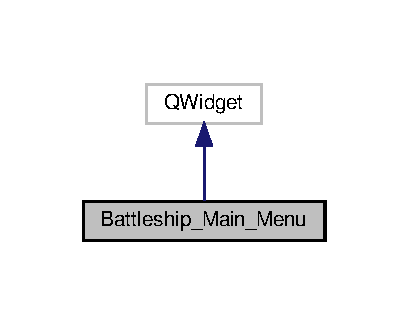
\includegraphics[width=196pt]{classBattleship__Main__Menu__inherit__graph}
\end{center}
\end{figure}


Collaboration diagram for Battleship\+\_\+\+Main\+\_\+\+Menu\+:\nopagebreak
\begin{figure}[H]
\begin{center}
\leavevmode
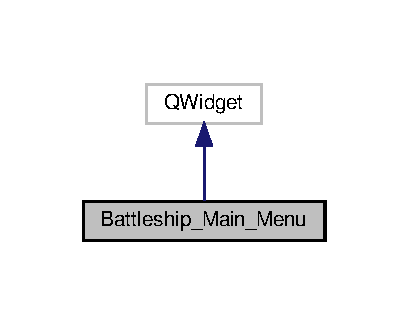
\includegraphics[width=196pt]{classBattleship__Main__Menu__coll__graph}
\end{center}
\end{figure}
\subsection*{Public Member Functions}
\begin{DoxyCompactItemize}
\item 
\mbox{\Hypertarget{classBattleship__Main__Menu_ac59c49406eacad237384883a5a661217}\label{classBattleship__Main__Menu_ac59c49406eacad237384883a5a661217}} 
{\bfseries Battleship\+\_\+\+Main\+\_\+\+Menu} (Q\+Widget $\ast$parent=nullptr)
\item 
\mbox{\Hypertarget{classBattleship__Main__Menu_ae8d3ea34b6127e1d0c5f7ec5fbe2fd46}\label{classBattleship__Main__Menu_ae8d3ea34b6127e1d0c5f7ec5fbe2fd46}} 
void \hyperlink{classBattleship__Main__Menu_ae8d3ea34b6127e1d0c5f7ec5fbe2fd46}{to\+\_\+new\+\_\+window\+\_\+key\+\_\+click} (Q\+Key\+Event $\ast$event)
\begin{DoxyCompactList}\small\item\em Function that takes the user to the battleship game when they click F1 key. \end{DoxyCompactList}\item 
void \hyperlink{classBattleship__Main__Menu_a0c52fabea744d8fa9397b6aa43ef7fb8}{get\+User} (Q\+String username)
\begin{DoxyCompactList}\small\item\em Function that retreives the name of the user. \end{DoxyCompactList}\end{DoxyCompactItemize}
\subsection*{Public Attributes}
\begin{DoxyCompactItemize}
\item 
\mbox{\Hypertarget{classBattleship__Main__Menu_a6773ebebe3d05284fc73d2cd33956be2}\label{classBattleship__Main__Menu_a6773ebebe3d05284fc73d2cd33956be2}} 
Q\+String {\bfseries menu\+\_\+username}
\end{DoxyCompactItemize}


\subsection{Member Function Documentation}
\mbox{\Hypertarget{classBattleship__Main__Menu_a0c52fabea744d8fa9397b6aa43ef7fb8}\label{classBattleship__Main__Menu_a0c52fabea744d8fa9397b6aa43ef7fb8}} 
\index{Battleship\+\_\+\+Main\+\_\+\+Menu@{Battleship\+\_\+\+Main\+\_\+\+Menu}!get\+User@{get\+User}}
\index{get\+User@{get\+User}!Battleship\+\_\+\+Main\+\_\+\+Menu@{Battleship\+\_\+\+Main\+\_\+\+Menu}}
\subsubsection{\texorpdfstring{get\+User()}{getUser()}}
{\footnotesize\ttfamily void Battleship\+\_\+\+Main\+\_\+\+Menu\+::get\+User (\begin{DoxyParamCaption}\item[{Q\+String}]{username }\end{DoxyParamCaption})}



Function that retreives the name of the user. 


\begin{DoxyParams}{Parameters}
{\em username} & \\
\hline
\end{DoxyParams}


The documentation for this class was generated from the following files\+:\begin{DoxyCompactItemize}
\item 
\hyperlink{battleship__main__menu_8h}{battleship\+\_\+main\+\_\+menu.\+h}\item 
\hyperlink{battleship__main__menu_8cpp}{battleship\+\_\+main\+\_\+menu.\+cpp}\end{DoxyCompactItemize}

\hypertarget{classgame2}{}\section{game2 Class Reference}
\label{classgame2}\index{game2@{game2}}


Inheritance diagram for game2\+:\nopagebreak
\begin{figure}[H]
\begin{center}
\leavevmode
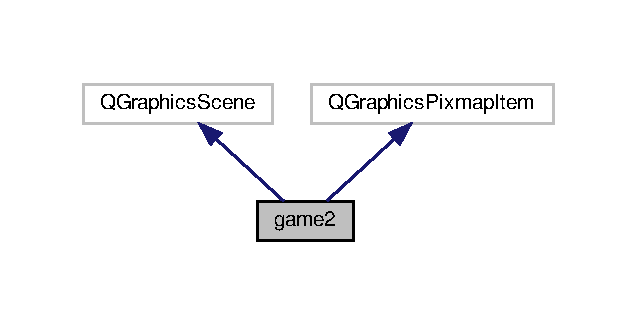
\includegraphics[width=306pt]{classgame2__inherit__graph}
\end{center}
\end{figure}


Collaboration diagram for game2\+:\nopagebreak
\begin{figure}[H]
\begin{center}
\leavevmode
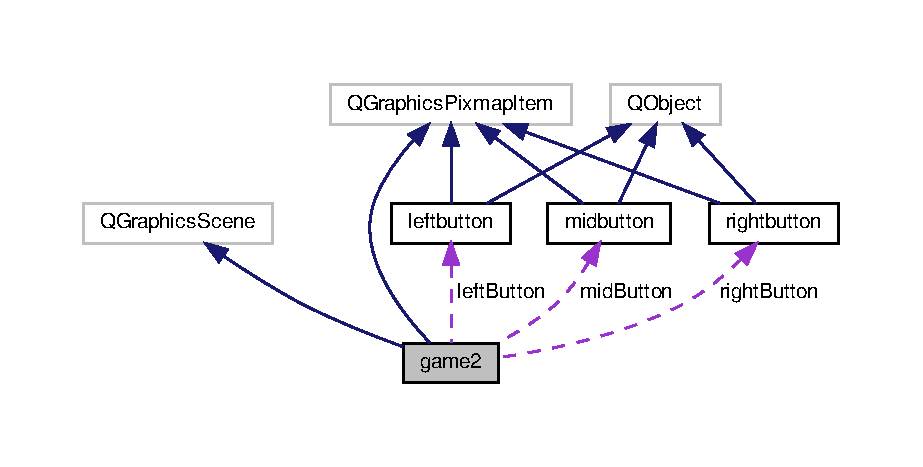
\includegraphics[width=350pt]{classgame2__coll__graph}
\end{center}
\end{figure}
\subsection*{Public Slots}
\begin{DoxyCompactItemize}
\item 
void \hyperlink{classgame2_a420782b0d5c32bf9960600a13a30c1f2}{create\+\_\+left} ()
\begin{DoxyCompactList}\small\item\em Function that creates discs in the left lane. \end{DoxyCompactList}\item 
void \hyperlink{classgame2_a6e5964212932ec9d08d5df31a93b3010}{create\+\_\+mid} ()
\begin{DoxyCompactList}\small\item\em Function that creates discs in the middle lane. \end{DoxyCompactList}\item 
void \hyperlink{classgame2_a1a554d82d02057789cfdfc8381bf5b4c}{create\+\_\+right} ()
\begin{DoxyCompactList}\small\item\em Function that creates discs in the right lane. \end{DoxyCompactList}\item 
void \hyperlink{classgame2_a8d1b4b72e005fb59df223b5df7757d43}{check\+Misses} ()
\begin{DoxyCompactList}\small\item\em Function that checks number of missed disks. \end{DoxyCompactList}\end{DoxyCompactItemize}
\subsection*{Public Member Functions}
\begin{DoxyCompactItemize}
\item 
\mbox{\Hypertarget{classgame2_a6ffa0bd5a0bc924421686b3a6951bdd4}\label{classgame2_a6ffa0bd5a0bc924421686b3a6951bdd4}} 
{\bfseries game2} (Q\+Graphics\+Scene $\ast$parent=nullptr)
\item 
\mbox{\Hypertarget{classgame2_a8c9e777d1909be0a2d5d9e7f96d65cf1}\label{classgame2_a8c9e777d1909be0a2d5d9e7f96d65cf1}} 
void {\bfseries key\+Press\+Event} (Q\+Key\+Event $\ast$event)
\end{DoxyCompactItemize}
\subsection*{Public Attributes}
\begin{DoxyCompactItemize}
\item 
\mbox{\Hypertarget{classgame2_a0375921b8927efec242f61d868de0c9a}\label{classgame2_a0375921b8927efec242f61d868de0c9a}} 
Q\+Label $\ast$ \hyperlink{classgame2_a0375921b8927efec242f61d868de0c9a}{counter\+\_\+label}
\begin{DoxyCompactList}\small\item\em Label to keep track of total score and display it. \end{DoxyCompactList}\item 
\mbox{\Hypertarget{classgame2_a6ee0d244c43062475f0c72eb9b698e46}\label{classgame2_a6ee0d244c43062475f0c72eb9b698e46}} 
Q\+Grid\+Layout $\ast$ \hyperlink{classgame2_a6ee0d244c43062475f0c72eb9b698e46}{background}
\begin{DoxyCompactList}\small\item\em Background of the game. \end{DoxyCompactList}\item 
\mbox{\Hypertarget{classgame2_abb0710dc45b20d3fa634616415dca500}\label{classgame2_abb0710dc45b20d3fa634616415dca500}} 
\hyperlink{classleftbutton}{leftbutton} $\ast$ {\bfseries left\+Button}
\item 
\mbox{\Hypertarget{classgame2_ae0df4aa49cf727c59bb9a82ec699b579}\label{classgame2_ae0df4aa49cf727c59bb9a82ec699b579}} 
\hyperlink{classrightbutton}{rightbutton} $\ast$ {\bfseries right\+Button}
\item 
\mbox{\Hypertarget{classgame2_a05923f1dd5bd72763730557ee472c438}\label{classgame2_a05923f1dd5bd72763730557ee472c438}} 
\hyperlink{classmidbutton}{midbutton} $\ast$ {\bfseries mid\+Button}
\item 
\mbox{\Hypertarget{classgame2_ab25b8f61e668504361a5146864a11aed}\label{classgame2_ab25b8f61e668504361a5146864a11aed}} 
Q\+Graphics\+View $\ast$ \hyperlink{classgame2_ab25b8f61e668504361a5146864a11aed}{view}
\begin{DoxyCompactList}\small\item\em Graphics View. \end{DoxyCompactList}\end{DoxyCompactItemize}


\subsection{Member Function Documentation}
\mbox{\Hypertarget{classgame2_a8d1b4b72e005fb59df223b5df7757d43}\label{classgame2_a8d1b4b72e005fb59df223b5df7757d43}} 
\index{game2@{game2}!check\+Misses@{check\+Misses}}
\index{check\+Misses@{check\+Misses}!game2@{game2}}
\subsubsection{\texorpdfstring{check\+Misses}{checkMisses}}
{\footnotesize\ttfamily void game2\+::check\+Misses (\begin{DoxyParamCaption}{ }\end{DoxyParamCaption})\hspace{0.3cm}{\ttfamily [slot]}}



Function that checks number of missed disks. 

Checks if number of missed disks is 3 to end the game \mbox{\Hypertarget{classgame2_a420782b0d5c32bf9960600a13a30c1f2}\label{classgame2_a420782b0d5c32bf9960600a13a30c1f2}} 
\index{game2@{game2}!create\+\_\+left@{create\+\_\+left}}
\index{create\+\_\+left@{create\+\_\+left}!game2@{game2}}
\subsubsection{\texorpdfstring{create\+\_\+left}{create\_left}}
{\footnotesize\ttfamily void game2\+::create\+\_\+left (\begin{DoxyParamCaption}{ }\end{DoxyParamCaption})\hspace{0.3cm}{\ttfamily [slot]}}



Function that creates discs in the left lane. 

This function creates discs in the left lane

It adjusts the speed at which the discs are created based on the score of the player

It starts at 1x speed, increases to 2x, then to 8x \mbox{\Hypertarget{classgame2_a6e5964212932ec9d08d5df31a93b3010}\label{classgame2_a6e5964212932ec9d08d5df31a93b3010}} 
\index{game2@{game2}!create\+\_\+mid@{create\+\_\+mid}}
\index{create\+\_\+mid@{create\+\_\+mid}!game2@{game2}}
\subsubsection{\texorpdfstring{create\+\_\+mid}{create\_mid}}
{\footnotesize\ttfamily void game2\+::create\+\_\+mid (\begin{DoxyParamCaption}{ }\end{DoxyParamCaption})\hspace{0.3cm}{\ttfamily [slot]}}



Function that creates discs in the middle lane. 

This function creates discs in the middle lane

It adjusts the speed at which the discs are created based on the score of the player

It starts at 1x speed, increases to 2x, then to 8x \mbox{\Hypertarget{classgame2_a1a554d82d02057789cfdfc8381bf5b4c}\label{classgame2_a1a554d82d02057789cfdfc8381bf5b4c}} 
\index{game2@{game2}!create\+\_\+right@{create\+\_\+right}}
\index{create\+\_\+right@{create\+\_\+right}!game2@{game2}}
\subsubsection{\texorpdfstring{create\+\_\+right}{create\_right}}
{\footnotesize\ttfamily void game2\+::create\+\_\+right (\begin{DoxyParamCaption}{ }\end{DoxyParamCaption})\hspace{0.3cm}{\ttfamily [slot]}}



Function that creates discs in the right lane. 

This function creates discs in the right lane

It adjusts the speed at which the discs are created based on the score of the player

It starts at 1x speed, increases to 2x, then to 8x 

The documentation for this class was generated from the following files\+:\begin{DoxyCompactItemize}
\item 
\hyperlink{game2_8h}{game2.\+h}\item 
\hyperlink{game2_8cpp}{game2.\+cpp}\end{DoxyCompactItemize}

\hypertarget{classgame2__main__menu}{}\section{game2\+\_\+main\+\_\+menu Class Reference}
\label{classgame2__main__menu}\index{game2\+\_\+main\+\_\+menu@{game2\+\_\+main\+\_\+menu}}


Inheritance diagram for game2\+\_\+main\+\_\+menu\+:\nopagebreak
\begin{figure}[H]
\begin{center}
\leavevmode
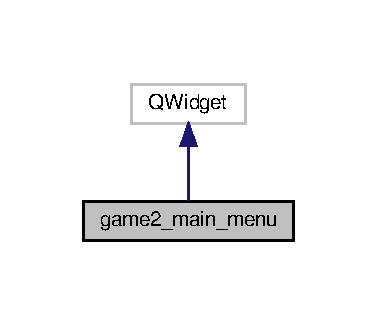
\includegraphics[width=181pt]{classgame2__main__menu__inherit__graph}
\end{center}
\end{figure}


Collaboration diagram for game2\+\_\+main\+\_\+menu\+:\nopagebreak
\begin{figure}[H]
\begin{center}
\leavevmode
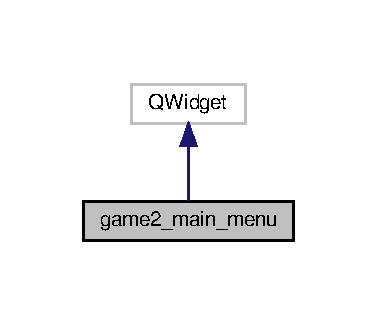
\includegraphics[width=181pt]{classgame2__main__menu__coll__graph}
\end{center}
\end{figure}
\subsection*{Public Member Functions}
\begin{DoxyCompactItemize}
\item 
\mbox{\Hypertarget{classgame2__main__menu_a012586b37247c91835178378b795945b}\label{classgame2__main__menu_a012586b37247c91835178378b795945b}} 
{\bfseries game2\+\_\+main\+\_\+menu} (Q\+Widget $\ast$parent=nullptr)
\item 
void \hyperlink{classgame2__main__menu_aa77f5a5ba961a25e6f9ed6112de186ad}{get\+User} (Q\+String username)
\begin{DoxyCompactList}\small\item\em Function that retreives username. \end{DoxyCompactList}\end{DoxyCompactItemize}
\subsection*{Public Attributes}
\begin{DoxyCompactItemize}
\item 
\mbox{\Hypertarget{classgame2__main__menu_a1da7101d69e9b4748d7d1c8a11c04edc}\label{classgame2__main__menu_a1da7101d69e9b4748d7d1c8a11c04edc}} 
Q\+Grid\+Layout $\ast$ \hyperlink{classgame2__main__menu_a1da7101d69e9b4748d7d1c8a11c04edc}{main\+\_\+menu}
\begin{DoxyCompactList}\small\item\em Grid for the main menu. \end{DoxyCompactList}\item 
\mbox{\Hypertarget{classgame2__main__menu_aa7c54c525cc6e3608cd2402195bb3d79}\label{classgame2__main__menu_aa7c54c525cc6e3608cd2402195bb3d79}} 
Q\+Push\+Button $\ast$ \hyperlink{classgame2__main__menu_aa7c54c525cc6e3608cd2402195bb3d79}{start}
\begin{DoxyCompactList}\small\item\em Start button. \end{DoxyCompactList}\item 
\mbox{\Hypertarget{classgame2__main__menu_a2ba46b5b8e3a389e3e46c6ab3a34febe}\label{classgame2__main__menu_a2ba46b5b8e3a389e3e46c6ab3a34febe}} 
Q\+String {\bfseries menu\+\_\+username}
\end{DoxyCompactItemize}


\subsection{Member Function Documentation}
\mbox{\Hypertarget{classgame2__main__menu_aa77f5a5ba961a25e6f9ed6112de186ad}\label{classgame2__main__menu_aa77f5a5ba961a25e6f9ed6112de186ad}} 
\index{game2\+\_\+main\+\_\+menu@{game2\+\_\+main\+\_\+menu}!get\+User@{get\+User}}
\index{get\+User@{get\+User}!game2\+\_\+main\+\_\+menu@{game2\+\_\+main\+\_\+menu}}
\subsubsection{\texorpdfstring{get\+User()}{getUser()}}
{\footnotesize\ttfamily void game2\+\_\+main\+\_\+menu\+::get\+User (\begin{DoxyParamCaption}\item[{Q\+String}]{username }\end{DoxyParamCaption})}



Function that retreives username. 



The documentation for this class was generated from the following files\+:\begin{DoxyCompactItemize}
\item 
\hyperlink{game2__main__menu_8h}{game2\+\_\+main\+\_\+menu.\+h}\item 
\hyperlink{game2__main__menu_8cpp}{game2\+\_\+main\+\_\+menu.\+cpp}\end{DoxyCompactItemize}

\hypertarget{classhistorypanel}{}\section{historypanel Class Reference}
\label{classhistorypanel}\index{historypanel@{historypanel}}


Inheritance diagram for historypanel\+:\nopagebreak
\begin{figure}[H]
\begin{center}
\leavevmode
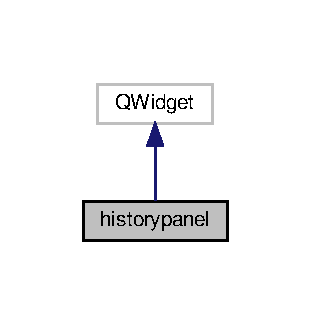
\includegraphics[width=149pt]{classhistorypanel__inherit__graph}
\end{center}
\end{figure}


Collaboration diagram for historypanel\+:\nopagebreak
\begin{figure}[H]
\begin{center}
\leavevmode
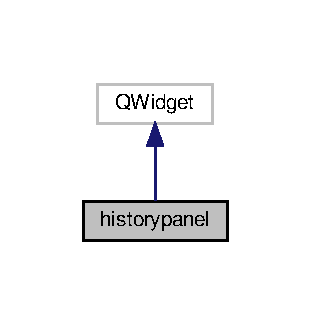
\includegraphics[width=149pt]{classhistorypanel__coll__graph}
\end{center}
\end{figure}
\subsection*{Public Slots}
\begin{DoxyCompactItemize}
\item 
\mbox{\Hypertarget{classhistorypanel_a93f8f39455d2465e5f4cb95d9e82cb65}\label{classhistorypanel_a93f8f39455d2465e5f4cb95d9e82cb65}} 
void \hyperlink{classhistorypanel_a93f8f39455d2465e5f4cb95d9e82cb65}{back} ()
\begin{DoxyCompactList}\small\item\em function to go back to previous panel \end{DoxyCompactList}\end{DoxyCompactItemize}
\subsection*{Public Member Functions}
\begin{DoxyCompactItemize}
\item 
\mbox{\Hypertarget{classhistorypanel_a59a94361f187f92f34526e865d3e8b63}\label{classhistorypanel_a59a94361f187f92f34526e865d3e8b63}} 
{\bfseries historypanel} (Q\+Widget $\ast$parent=nullptr)
\item 
\mbox{\Hypertarget{classhistorypanel_ae0e1b47118a187d381bc40aff467e1d6}\label{classhistorypanel_ae0e1b47118a187d381bc40aff467e1d6}} 
void {\bfseries get\+History} (Q\+String)
\end{DoxyCompactItemize}


The documentation for this class was generated from the following files\+:\begin{DoxyCompactItemize}
\item 
\hyperlink{historypanel_8h}{historypanel.\+h}\item 
\hyperlink{historypanel_8cpp}{historypanel.\+cpp}\end{DoxyCompactItemize}

\hypertarget{classleft__disks}{}\section{left\+\_\+disks Class Reference}
\label{classleft__disks}\index{left\+\_\+disks@{left\+\_\+disks}}


Inheritance diagram for left\+\_\+disks\+:\nopagebreak
\begin{figure}[H]
\begin{center}
\leavevmode
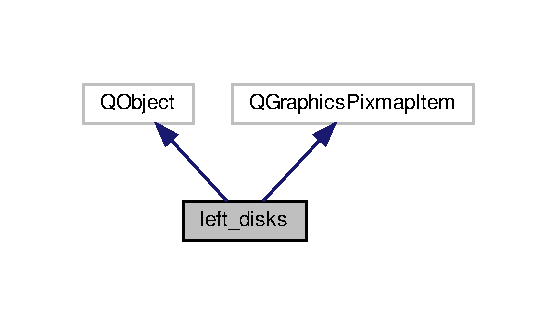
\includegraphics[width=268pt]{classleft__disks__inherit__graph}
\end{center}
\end{figure}


Collaboration diagram for left\+\_\+disks\+:\nopagebreak
\begin{figure}[H]
\begin{center}
\leavevmode
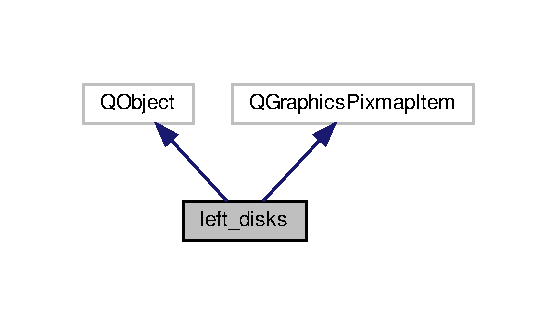
\includegraphics[width=268pt]{classleft__disks__coll__graph}
\end{center}
\end{figure}
\subsection*{Public Slots}
\begin{DoxyCompactItemize}
\item 
void \hyperlink{classleft__disks_a613675662c3b7d427671ca6aa2aa4fc4}{update} ()
\begin{DoxyCompactList}\small\item\em Function that updates the position of left discs. \end{DoxyCompactList}\end{DoxyCompactItemize}
\subsection*{Public Member Functions}
\begin{DoxyCompactItemize}
\item 
\mbox{\Hypertarget{classleft__disks_a45551856594caed4f92a81a4a4d7bd4d}\label{classleft__disks_a45551856594caed4f92a81a4a4d7bd4d}} 
{\bfseries left\+\_\+disks} (Q\+Object $\ast$parent=0)
\end{DoxyCompactItemize}


\subsection{Member Function Documentation}
\mbox{\Hypertarget{classleft__disks_a613675662c3b7d427671ca6aa2aa4fc4}\label{classleft__disks_a613675662c3b7d427671ca6aa2aa4fc4}} 
\index{left\+\_\+disks@{left\+\_\+disks}!update@{update}}
\index{update@{update}!left\+\_\+disks@{left\+\_\+disks}}
\subsubsection{\texorpdfstring{update}{update}}
{\footnotesize\ttfamily void left\+\_\+disks\+::update (\begin{DoxyParamCaption}{ }\end{DoxyParamCaption})\hspace{0.3cm}{\ttfamily [slot]}}



Function that updates the position of left discs. 

This function updates the x,y position of a left disc on screen

The function also checks the y() position of a disc and increments missed\+\_\+disks if that y() position is above a certain value 

The documentation for this class was generated from the following files\+:\begin{DoxyCompactItemize}
\item 
\hyperlink{left__disks_8h}{left\+\_\+disks.\+h}\item 
\hyperlink{left__disks_8cpp}{left\+\_\+disks.\+cpp}\end{DoxyCompactItemize}

\hypertarget{classleftbutton}{}\section{leftbutton Class Reference}
\label{classleftbutton}\index{leftbutton@{leftbutton}}


Inheritance diagram for leftbutton\+:\nopagebreak
\begin{figure}[H]
\begin{center}
\leavevmode
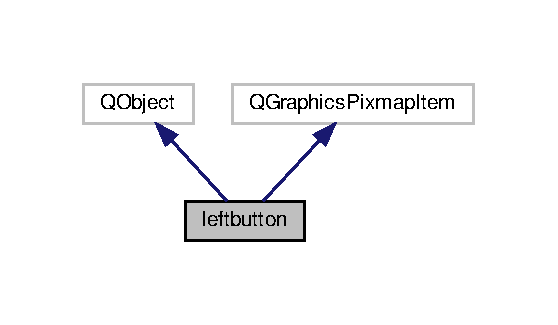
\includegraphics[width=268pt]{classleftbutton__inherit__graph}
\end{center}
\end{figure}


Collaboration diagram for leftbutton\+:\nopagebreak
\begin{figure}[H]
\begin{center}
\leavevmode
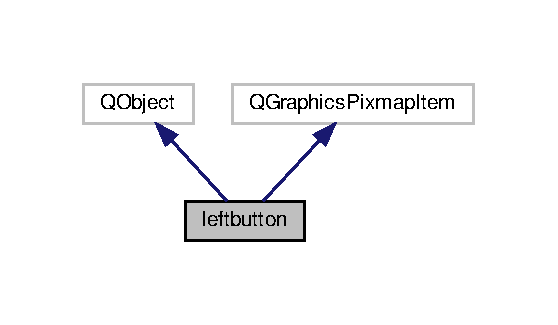
\includegraphics[width=268pt]{classleftbutton__coll__graph}
\end{center}
\end{figure}
\subsection*{Public Member Functions}
\begin{DoxyCompactItemize}
\item 
\mbox{\Hypertarget{classleftbutton_a2ba51e2ca7ed0afa9fcab8cd4bd44479}\label{classleftbutton_a2ba51e2ca7ed0afa9fcab8cd4bd44479}} 
{\bfseries leftbutton} (Q\+Object $\ast$parent=0)
\item 
bool \hyperlink{classleftbutton_a33d7fbc6aff28b0233286d3c99c79e83}{check\+Coll} ()
\begin{DoxyCompactList}\small\item\em Function that checks collision between left button and objects (discs) \end{DoxyCompactList}\end{DoxyCompactItemize}


\subsection{Member Function Documentation}
\mbox{\Hypertarget{classleftbutton_a33d7fbc6aff28b0233286d3c99c79e83}\label{classleftbutton_a33d7fbc6aff28b0233286d3c99c79e83}} 
\index{leftbutton@{leftbutton}!check\+Coll@{check\+Coll}}
\index{check\+Coll@{check\+Coll}!leftbutton@{leftbutton}}
\subsubsection{\texorpdfstring{check\+Coll()}{checkColl()}}
{\footnotesize\ttfamily bool leftbutton\+::check\+Coll (\begin{DoxyParamCaption}{ }\end{DoxyParamCaption})}



Function that checks collision between left button and objects (discs) 

\begin{DoxyReturn}{Returns}
bool\+: true if there was collision, false otherwise 
\end{DoxyReturn}


The documentation for this class was generated from the following files\+:\begin{DoxyCompactItemize}
\item 
\hyperlink{leftbutton_8h}{leftbutton.\+h}\item 
\hyperlink{leftbutton_8cpp}{leftbutton.\+cpp}\end{DoxyCompactItemize}

\hypertarget{classloginPanel}{}\section{login\+Panel Class Reference}
\label{classloginPanel}\index{login\+Panel@{login\+Panel}}


Inheritance diagram for login\+Panel\+:\nopagebreak
\begin{figure}[H]
\begin{center}
\leavevmode
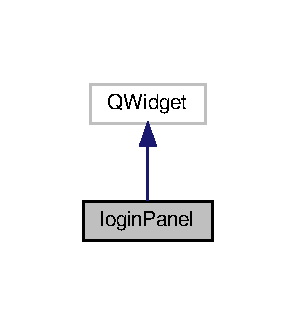
\includegraphics[width=142pt]{classloginPanel__inherit__graph}
\end{center}
\end{figure}


Collaboration diagram for login\+Panel\+:\nopagebreak
\begin{figure}[H]
\begin{center}
\leavevmode
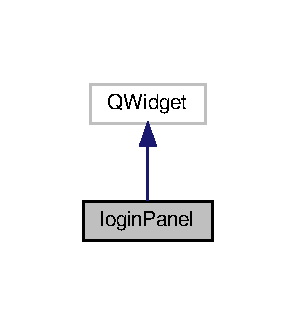
\includegraphics[width=142pt]{classloginPanel__coll__graph}
\end{center}
\end{figure}
\subsection*{Public Member Functions}
\begin{DoxyCompactItemize}
\item 
\mbox{\Hypertarget{classloginPanel_a22f12ed558377b1de1738117419c6e6e}\label{classloginPanel_a22f12ed558377b1de1738117419c6e6e}} 
{\bfseries login\+Panel} (Q\+Widget $\ast$parent=nullptr)
\end{DoxyCompactItemize}


The documentation for this class was generated from the following files\+:\begin{DoxyCompactItemize}
\item 
\hyperlink{loginpanel_8h}{loginpanel.\+h}\item 
\hyperlink{loginpanel_8cpp}{loginpanel.\+cpp}\end{DoxyCompactItemize}

\hypertarget{classlose__screen}{}\section{lose\+\_\+screen Class Reference}
\label{classlose__screen}\index{lose\+\_\+screen@{lose\+\_\+screen}}


Inheritance diagram for lose\+\_\+screen\+:\nopagebreak
\begin{figure}[H]
\begin{center}
\leavevmode
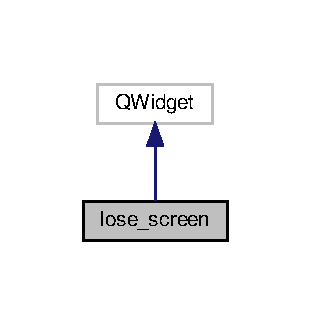
\includegraphics[width=149pt]{classlose__screen__inherit__graph}
\end{center}
\end{figure}


Collaboration diagram for lose\+\_\+screen\+:\nopagebreak
\begin{figure}[H]
\begin{center}
\leavevmode
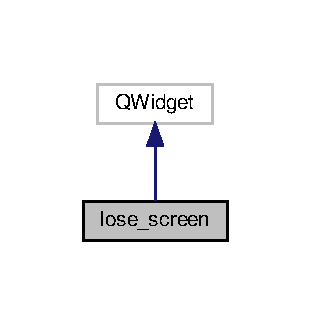
\includegraphics[width=149pt]{classlose__screen__coll__graph}
\end{center}
\end{figure}
\subsection*{Public Member Functions}
\begin{DoxyCompactItemize}
\item 
\mbox{\Hypertarget{classlose__screen_a4f8848074280e3ea90ab9f6c6c66852a}\label{classlose__screen_a4f8848074280e3ea90ab9f6c6c66852a}} 
{\bfseries lose\+\_\+screen} (Q\+Widget $\ast$parent=nullptr)
\end{DoxyCompactItemize}
\subsection*{Public Attributes}
\begin{DoxyCompactItemize}
\item 
\mbox{\Hypertarget{classlose__screen_af9115788ae21e6456809d84e0f49e703}\label{classlose__screen_af9115788ae21e6456809d84e0f49e703}} 
Q\+Grid\+Layout $\ast$ {\bfseries grid}
\item 
\mbox{\Hypertarget{classlose__screen_ac5b40c4bce6f5047658ca80059aa4400}\label{classlose__screen_ac5b40c4bce6f5047658ca80059aa4400}} 
Q\+Label $\ast$ {\bfseries lose}
\item 
\mbox{\Hypertarget{classlose__screen_a28c2c0d39d940edd66962907f78da527}\label{classlose__screen_a28c2c0d39d940edd66962907f78da527}} 
Q\+Push\+Button $\ast$ {\bfseries return\+\_\+to\+\_\+login}
\end{DoxyCompactItemize}


The documentation for this class was generated from the following files\+:\begin{DoxyCompactItemize}
\item 
\hyperlink{lose__screen_8h}{lose\+\_\+screen.\+h}\item 
\hyperlink{lose__screen_8cpp}{lose\+\_\+screen.\+cpp}\end{DoxyCompactItemize}

\hypertarget{classmainpanel}{}\section{mainpanel Class Reference}
\label{classmainpanel}\index{mainpanel@{mainpanel}}


Inheritance diagram for mainpanel\+:\nopagebreak
\begin{figure}[H]
\begin{center}
\leavevmode
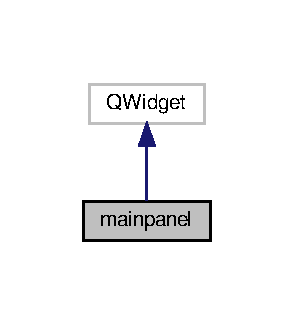
\includegraphics[width=141pt]{classmainpanel__inherit__graph}
\end{center}
\end{figure}


Collaboration diagram for mainpanel\+:\nopagebreak
\begin{figure}[H]
\begin{center}
\leavevmode
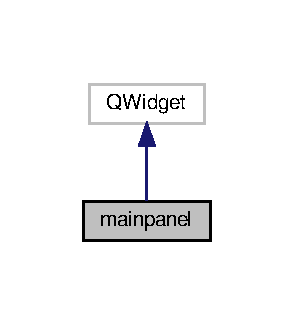
\includegraphics[width=141pt]{classmainpanel__coll__graph}
\end{center}
\end{figure}
\subsection*{Public Member Functions}
\begin{DoxyCompactItemize}
\item 
\mbox{\Hypertarget{classmainpanel_a20d907a14bc430ffdc6cedfbccf8705a}\label{classmainpanel_a20d907a14bc430ffdc6cedfbccf8705a}} 
{\bfseries mainpanel} (Q\+Widget $\ast$parent=nullptr)
\end{DoxyCompactItemize}


The documentation for this class was generated from the following files\+:\begin{DoxyCompactItemize}
\item 
\hyperlink{mainpanel_8h}{mainpanel.\+h}\item 
\hyperlink{mainpanel_8cpp}{mainpanel.\+cpp}\end{DoxyCompactItemize}

\hypertarget{classmid__disks}{}\section{mid\+\_\+disks Class Reference}
\label{classmid__disks}\index{mid\+\_\+disks@{mid\+\_\+disks}}


Inheritance diagram for mid\+\_\+disks\+:\nopagebreak
\begin{figure}[H]
\begin{center}
\leavevmode
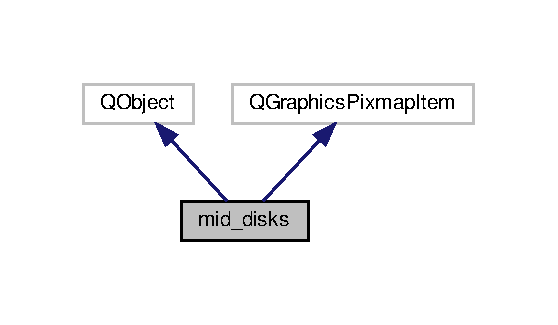
\includegraphics[width=268pt]{classmid__disks__inherit__graph}
\end{center}
\end{figure}


Collaboration diagram for mid\+\_\+disks\+:\nopagebreak
\begin{figure}[H]
\begin{center}
\leavevmode
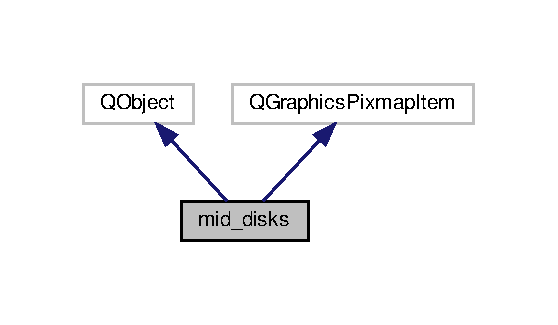
\includegraphics[width=268pt]{classmid__disks__coll__graph}
\end{center}
\end{figure}
\subsection*{Public Slots}
\begin{DoxyCompactItemize}
\item 
void \hyperlink{classmid__disks_aaf3ee8a13a79381553589e54b92b691c}{update} ()
\begin{DoxyCompactList}\small\item\em Function that updates the position of mid discs. \end{DoxyCompactList}\end{DoxyCompactItemize}
\subsection*{Public Member Functions}
\begin{DoxyCompactItemize}
\item 
\mbox{\Hypertarget{classmid__disks_a2a283183a343ba601007b002354d59cd}\label{classmid__disks_a2a283183a343ba601007b002354d59cd}} 
{\bfseries mid\+\_\+disks} (Q\+Object $\ast$parent=0)
\end{DoxyCompactItemize}


\subsection{Member Function Documentation}
\mbox{\Hypertarget{classmid__disks_aaf3ee8a13a79381553589e54b92b691c}\label{classmid__disks_aaf3ee8a13a79381553589e54b92b691c}} 
\index{mid\+\_\+disks@{mid\+\_\+disks}!update@{update}}
\index{update@{update}!mid\+\_\+disks@{mid\+\_\+disks}}
\subsubsection{\texorpdfstring{update}{update}}
{\footnotesize\ttfamily void mid\+\_\+disks\+::update (\begin{DoxyParamCaption}{ }\end{DoxyParamCaption})\hspace{0.3cm}{\ttfamily [slot]}}



Function that updates the position of mid discs. 

This function updates the x,y position of a mid disc on screen

The function also checks the y() position of a disc and increments missed\+\_\+disks if that y() position is above a certain value 

The documentation for this class was generated from the following files\+:\begin{DoxyCompactItemize}
\item 
\hyperlink{mid__disks_8h}{mid\+\_\+disks.\+h}\item 
\hyperlink{mid__disks_8cpp}{mid\+\_\+disks.\+cpp}\end{DoxyCompactItemize}

\hypertarget{classmidbutton}{}\section{midbutton Class Reference}
\label{classmidbutton}\index{midbutton@{midbutton}}


Inheritance diagram for midbutton\+:\nopagebreak
\begin{figure}[H]
\begin{center}
\leavevmode
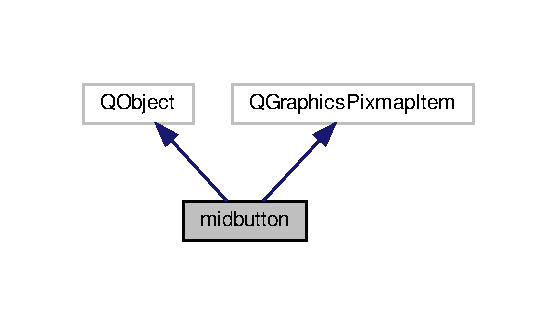
\includegraphics[width=268pt]{classmidbutton__inherit__graph}
\end{center}
\end{figure}


Collaboration diagram for midbutton\+:\nopagebreak
\begin{figure}[H]
\begin{center}
\leavevmode
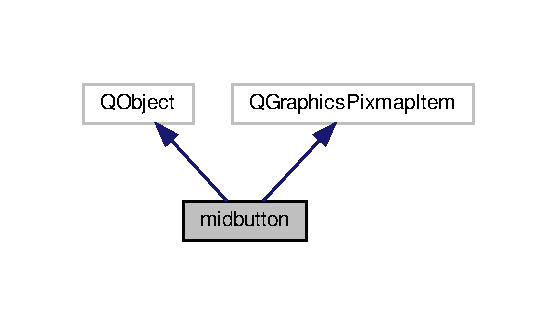
\includegraphics[width=268pt]{classmidbutton__coll__graph}
\end{center}
\end{figure}
\subsection*{Public Member Functions}
\begin{DoxyCompactItemize}
\item 
\mbox{\Hypertarget{classmidbutton_a18399a4d013722bf7df021ef68f0df7c}\label{classmidbutton_a18399a4d013722bf7df021ef68f0df7c}} 
{\bfseries midbutton} (Q\+Object $\ast$parent=nullptr)
\item 
bool \hyperlink{classmidbutton_a6a711973ae7e7d0a3d98f0581130521d}{check\+Coll} ()
\begin{DoxyCompactList}\small\item\em Function that checks collision between mid button and objects (discs) \end{DoxyCompactList}\end{DoxyCompactItemize}


\subsection{Member Function Documentation}
\mbox{\Hypertarget{classmidbutton_a6a711973ae7e7d0a3d98f0581130521d}\label{classmidbutton_a6a711973ae7e7d0a3d98f0581130521d}} 
\index{midbutton@{midbutton}!check\+Coll@{check\+Coll}}
\index{check\+Coll@{check\+Coll}!midbutton@{midbutton}}
\subsubsection{\texorpdfstring{check\+Coll()}{checkColl()}}
{\footnotesize\ttfamily bool midbutton\+::check\+Coll (\begin{DoxyParamCaption}{ }\end{DoxyParamCaption})}



Function that checks collision between mid button and objects (discs) 

\begin{DoxyReturn}{Returns}
bool\+: true if there was collision, false otherwise 
\end{DoxyReturn}


The documentation for this class was generated from the following files\+:\begin{DoxyCompactItemize}
\item 
\hyperlink{midbutton_8h}{midbutton.\+h}\item 
\hyperlink{midbutton_8cpp}{midbutton.\+cpp}\end{DoxyCompactItemize}

\hypertarget{classquestion__tab}{}\section{question\+\_\+tab Class Reference}
\label{classquestion__tab}\index{question\+\_\+tab@{question\+\_\+tab}}


Inheritance diagram for question\+\_\+tab\+:\nopagebreak
\begin{figure}[H]
\begin{center}
\leavevmode
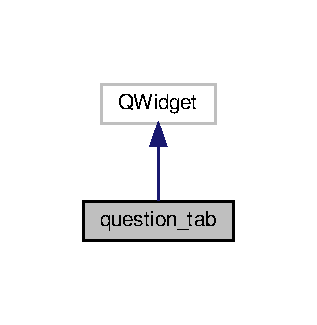
\includegraphics[width=152pt]{classquestion__tab__inherit__graph}
\end{center}
\end{figure}


Collaboration diagram for question\+\_\+tab\+:\nopagebreak
\begin{figure}[H]
\begin{center}
\leavevmode
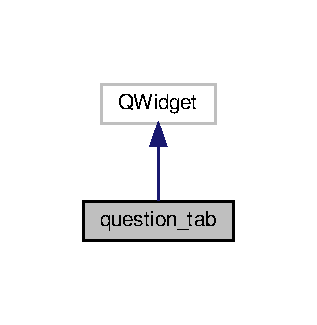
\includegraphics[width=152pt]{classquestion__tab__coll__graph}
\end{center}
\end{figure}
\subsection*{Public Member Functions}
\begin{DoxyCompactItemize}
\item 
\mbox{\Hypertarget{classquestion__tab_a22107ddfe29017c10a294c3f42d7c201}\label{classquestion__tab_a22107ddfe29017c10a294c3f42d7c201}} 
{\bfseries question\+\_\+tab} (Q\+Widget $\ast$parent=nullptr)
\end{DoxyCompactItemize}


The documentation for this class was generated from the following files\+:\begin{DoxyCompactItemize}
\item 
question\+\_\+tab.\+h\item 
question\+\_\+tab.\+cpp\end{DoxyCompactItemize}

\hypertarget{classright__disks}{}\section{right\+\_\+disks Class Reference}
\label{classright__disks}\index{right\+\_\+disks@{right\+\_\+disks}}


Inheritance diagram for right\+\_\+disks\+:\nopagebreak
\begin{figure}[H]
\begin{center}
\leavevmode
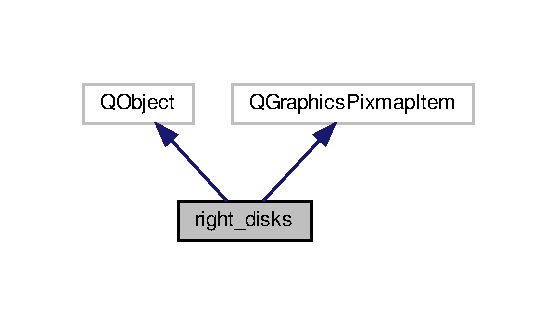
\includegraphics[width=268pt]{classright__disks__inherit__graph}
\end{center}
\end{figure}


Collaboration diagram for right\+\_\+disks\+:\nopagebreak
\begin{figure}[H]
\begin{center}
\leavevmode
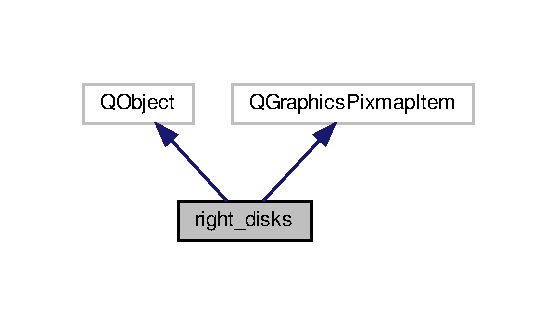
\includegraphics[width=268pt]{classright__disks__coll__graph}
\end{center}
\end{figure}
\subsection*{Public Slots}
\begin{DoxyCompactItemize}
\item 
void \hyperlink{classright__disks_a2dae29bf05aef3c3171d57f2aa7fa33f}{update} ()
\begin{DoxyCompactList}\small\item\em Function that updates the position of right discs. \end{DoxyCompactList}\end{DoxyCompactItemize}
\subsection*{Public Member Functions}
\begin{DoxyCompactItemize}
\item 
\mbox{\Hypertarget{classright__disks_a88cf720f84861003d8a31f08344228bc}\label{classright__disks_a88cf720f84861003d8a31f08344228bc}} 
{\bfseries right\+\_\+disks} (Q\+Object $\ast$parent=0)
\end{DoxyCompactItemize}


\subsection{Member Function Documentation}
\mbox{\Hypertarget{classright__disks_a2dae29bf05aef3c3171d57f2aa7fa33f}\label{classright__disks_a2dae29bf05aef3c3171d57f2aa7fa33f}} 
\index{right\+\_\+disks@{right\+\_\+disks}!update@{update}}
\index{update@{update}!right\+\_\+disks@{right\+\_\+disks}}
\subsubsection{\texorpdfstring{update}{update}}
{\footnotesize\ttfamily void right\+\_\+disks\+::update (\begin{DoxyParamCaption}{ }\end{DoxyParamCaption})\hspace{0.3cm}{\ttfamily [slot]}}



Function that updates the position of right discs. 

This function updates the x,y position of a right disc on screen

The function also checks the y() position of a disc and increments missed\+\_\+disks if that y() position is above a certain value 

The documentation for this class was generated from the following files\+:\begin{DoxyCompactItemize}
\item 
\hyperlink{right__disks_8h}{right\+\_\+disks.\+h}\item 
right\+\_\+disks.\+cpp\end{DoxyCompactItemize}

\hypertarget{classrightbutton}{}\section{rightbutton Class Reference}
\label{classrightbutton}\index{rightbutton@{rightbutton}}


Inheritance diagram for rightbutton\+:\nopagebreak
\begin{figure}[H]
\begin{center}
\leavevmode
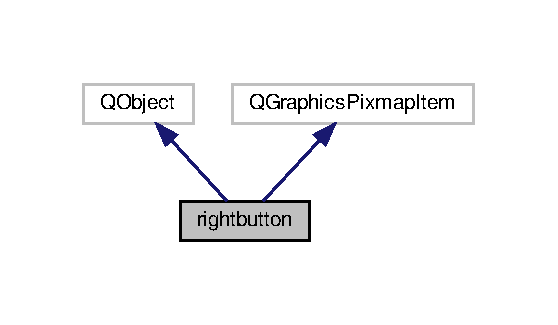
\includegraphics[width=268pt]{classrightbutton__inherit__graph}
\end{center}
\end{figure}


Collaboration diagram for rightbutton\+:\nopagebreak
\begin{figure}[H]
\begin{center}
\leavevmode
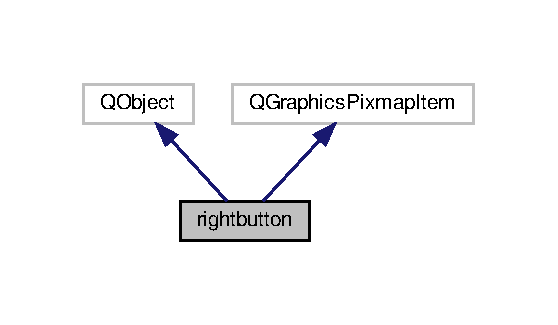
\includegraphics[width=268pt]{classrightbutton__coll__graph}
\end{center}
\end{figure}
\subsection*{Public Member Functions}
\begin{DoxyCompactItemize}
\item 
\mbox{\Hypertarget{classrightbutton_ae516758294d5cada4b99936e72aa9891}\label{classrightbutton_ae516758294d5cada4b99936e72aa9891}} 
{\bfseries rightbutton} (Q\+Object $\ast$parent=nullptr)
\item 
bool \hyperlink{classrightbutton_a50b7acc734df9c1e17e2acd718ba4ee9}{check\+Coll} ()
\begin{DoxyCompactList}\small\item\em Function that checks collision between right button and objects (discs) \end{DoxyCompactList}\end{DoxyCompactItemize}


\subsection{Member Function Documentation}
\mbox{\Hypertarget{classrightbutton_a50b7acc734df9c1e17e2acd718ba4ee9}\label{classrightbutton_a50b7acc734df9c1e17e2acd718ba4ee9}} 
\index{rightbutton@{rightbutton}!check\+Coll@{check\+Coll}}
\index{check\+Coll@{check\+Coll}!rightbutton@{rightbutton}}
\subsubsection{\texorpdfstring{check\+Coll()}{checkColl()}}
{\footnotesize\ttfamily bool rightbutton\+::check\+Coll (\begin{DoxyParamCaption}{ }\end{DoxyParamCaption})}



Function that checks collision between right button and objects (discs) 

\begin{DoxyReturn}{Returns}
bool\+: true if there was collision, false otherwise 
\end{DoxyReturn}


The documentation for this class was generated from the following files\+:\begin{DoxyCompactItemize}
\item 
\hyperlink{rightbutton_8h}{rightbutton.\+h}\item 
rightbutton.\+cpp\end{DoxyCompactItemize}

\hypertarget{classsignup__form}{}\section{signup\+\_\+form Class Reference}
\label{classsignup__form}\index{signup\+\_\+form@{signup\+\_\+form}}


Inheritance diagram for signup\+\_\+form\+:\nopagebreak
\begin{figure}[H]
\begin{center}
\leavevmode
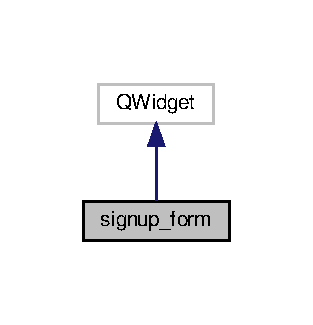
\includegraphics[width=150pt]{classsignup__form__inherit__graph}
\end{center}
\end{figure}


Collaboration diagram for signup\+\_\+form\+:\nopagebreak
\begin{figure}[H]
\begin{center}
\leavevmode
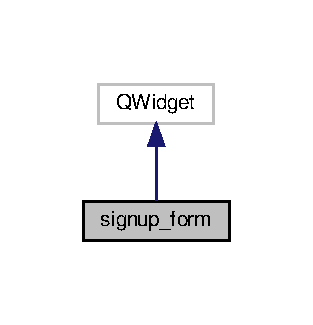
\includegraphics[width=150pt]{classsignup__form__coll__graph}
\end{center}
\end{figure}
\subsection*{Public Slots}
\begin{DoxyCompactItemize}
\item 
void \hyperlink{classsignup__form_a8d618167178f15d27937127a4a0efbc1}{check\+\_\+pass\+\_\+num\+\_\+empty} ()
\begin{DoxyCompactList}\small\item\em Function that checks if pass and phone number meet requirements. \end{DoxyCompactList}\item 
void \hyperlink{classsignup__form_a8fb6be94fb91979a3da75be5e123c4e7}{back\+\_\+from\+\_\+signup} ()
\begin{DoxyCompactList}\small\item\em Function that takes user back to main panel. \end{DoxyCompactList}\item 
void \hyperlink{classsignup__form_a919a6d06a8b45ec3672341d840572a0f}{select\+\_\+display\+\_\+image} ()
\begin{DoxyCompactList}\small\item\em Function that displays image selection. \end{DoxyCompactList}\item 
static bool \hyperlink{classsignup__form_aa1378656be593cc119db637e317a699c}{is\+Unique} (Q\+String curr\+\_\+name)
\begin{DoxyCompactList}\small\item\em Function that checks if username is unique. \end{DoxyCompactList}\end{DoxyCompactItemize}
\subsection*{Public Member Functions}
\begin{DoxyCompactItemize}
\item 
\mbox{\Hypertarget{classsignup__form_a3f0b23c1cc03c4c3800b9922716ffb35}\label{classsignup__form_a3f0b23c1cc03c4c3800b9922716ffb35}} 
{\bfseries signup\+\_\+form} (Q\+Widget $\ast$parent=nullptr)
\end{DoxyCompactItemize}


\subsection{Member Function Documentation}
\mbox{\Hypertarget{classsignup__form_a8fb6be94fb91979a3da75be5e123c4e7}\label{classsignup__form_a8fb6be94fb91979a3da75be5e123c4e7}} 
\index{signup\+\_\+form@{signup\+\_\+form}!back\+\_\+from\+\_\+signup@{back\+\_\+from\+\_\+signup}}
\index{back\+\_\+from\+\_\+signup@{back\+\_\+from\+\_\+signup}!signup\+\_\+form@{signup\+\_\+form}}
\subsubsection{\texorpdfstring{back\+\_\+from\+\_\+signup}{back\_from\_signup}}
{\footnotesize\ttfamily void signup\+\_\+form\+::back\+\_\+from\+\_\+signup (\begin{DoxyParamCaption}{ }\end{DoxyParamCaption})\hspace{0.3cm}{\ttfamily [slot]}}



Function that takes user back to main panel. 

\mbox{\Hypertarget{classsignup__form_a8d618167178f15d27937127a4a0efbc1}\label{classsignup__form_a8d618167178f15d27937127a4a0efbc1}} 
\index{signup\+\_\+form@{signup\+\_\+form}!check\+\_\+pass\+\_\+num\+\_\+empty@{check\+\_\+pass\+\_\+num\+\_\+empty}}
\index{check\+\_\+pass\+\_\+num\+\_\+empty@{check\+\_\+pass\+\_\+num\+\_\+empty}!signup\+\_\+form@{signup\+\_\+form}}
\subsubsection{\texorpdfstring{check\+\_\+pass\+\_\+num\+\_\+empty}{check\_pass\_num\_empty}}
{\footnotesize\ttfamily void signup\+\_\+form\+::check\+\_\+pass\+\_\+num\+\_\+empty (\begin{DoxyParamCaption}{ }\end{DoxyParamCaption})\hspace{0.3cm}{\ttfamily [slot]}}



Function that checks if pass and phone number meet requirements. 

\mbox{\Hypertarget{classsignup__form_aa1378656be593cc119db637e317a699c}\label{classsignup__form_aa1378656be593cc119db637e317a699c}} 
\index{signup\+\_\+form@{signup\+\_\+form}!is\+Unique@{is\+Unique}}
\index{is\+Unique@{is\+Unique}!signup\+\_\+form@{signup\+\_\+form}}
\subsubsection{\texorpdfstring{is\+Unique}{isUnique}}
{\footnotesize\ttfamily bool signup\+\_\+form\+::is\+Unique (\begin{DoxyParamCaption}\item[{Q\+String}]{curr\+\_\+name }\end{DoxyParamCaption})\hspace{0.3cm}{\ttfamily [static]}, {\ttfamily [slot]}}



Function that checks if username is unique. 

\mbox{\Hypertarget{classsignup__form_a919a6d06a8b45ec3672341d840572a0f}\label{classsignup__form_a919a6d06a8b45ec3672341d840572a0f}} 
\index{signup\+\_\+form@{signup\+\_\+form}!select\+\_\+display\+\_\+image@{select\+\_\+display\+\_\+image}}
\index{select\+\_\+display\+\_\+image@{select\+\_\+display\+\_\+image}!signup\+\_\+form@{signup\+\_\+form}}
\subsubsection{\texorpdfstring{select\+\_\+display\+\_\+image}{select\_display\_image}}
{\footnotesize\ttfamily void signup\+\_\+form\+::select\+\_\+display\+\_\+image (\begin{DoxyParamCaption}{ }\end{DoxyParamCaption})\hspace{0.3cm}{\ttfamily [slot]}}



Function that displays image selection. 



The documentation for this class was generated from the following files\+:\begin{DoxyCompactItemize}
\item 
\hyperlink{signup__form_8h}{signup\+\_\+form.\+h}\item 
\hyperlink{signup__form_8cpp}{signup\+\_\+form.\+cpp}\end{DoxyCompactItemize}

\hypertarget{classvictory__screen}{}\section{victory\+\_\+screen Class Reference}
\label{classvictory__screen}\index{victory\+\_\+screen@{victory\+\_\+screen}}


Inheritance diagram for victory\+\_\+screen\+:\nopagebreak
\begin{figure}[H]
\begin{center}
\leavevmode
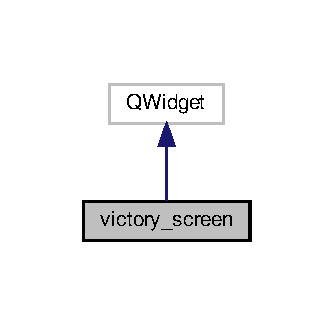
\includegraphics[width=160pt]{classvictory__screen__inherit__graph}
\end{center}
\end{figure}


Collaboration diagram for victory\+\_\+screen\+:\nopagebreak
\begin{figure}[H]
\begin{center}
\leavevmode
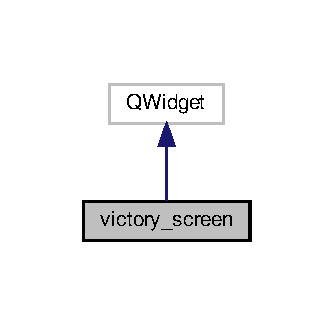
\includegraphics[width=160pt]{classvictory__screen__coll__graph}
\end{center}
\end{figure}
\subsection*{Public Member Functions}
\begin{DoxyCompactItemize}
\item 
\mbox{\Hypertarget{classvictory__screen_a5e81e9d86f259ff268b5bc3a3939817b}\label{classvictory__screen_a5e81e9d86f259ff268b5bc3a3939817b}} 
{\bfseries victory\+\_\+screen} (Q\+Widget $\ast$parent=nullptr)
\end{DoxyCompactItemize}


The documentation for this class was generated from the following files\+:\begin{DoxyCompactItemize}
\item 
\hyperlink{victory__screen_8h}{victory\+\_\+screen.\+h}\item 
\hyperlink{victory__screen_8cpp}{victory\+\_\+screen.\+cpp}\end{DoxyCompactItemize}

\hypertarget{classwelcome__screen}{}\section{welcome\+\_\+screen Class Reference}
\label{classwelcome__screen}\index{welcome\+\_\+screen@{welcome\+\_\+screen}}


Inheritance diagram for welcome\+\_\+screen\+:\nopagebreak
\begin{figure}[H]
\begin{center}
\leavevmode
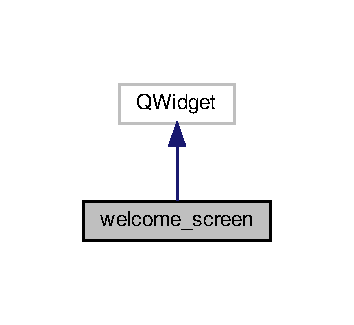
\includegraphics[width=170pt]{classwelcome__screen__inherit__graph}
\end{center}
\end{figure}


Collaboration diagram for welcome\+\_\+screen\+:\nopagebreak
\begin{figure}[H]
\begin{center}
\leavevmode
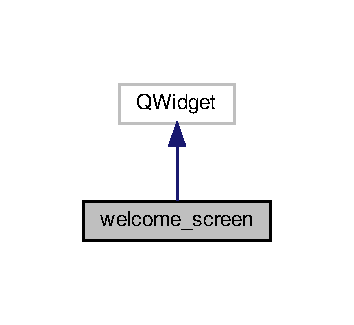
\includegraphics[width=170pt]{classwelcome__screen__coll__graph}
\end{center}
\end{figure}
\subsection*{Public Slots}
\begin{DoxyCompactItemize}
\item 
\mbox{\Hypertarget{classwelcome__screen_a9b00fa23427b130623c72f431c8ba2b0}\label{classwelcome__screen_a9b00fa23427b130623c72f431c8ba2b0}} 
void \hyperlink{classwelcome__screen_a9b00fa23427b130623c72f431c8ba2b0}{back\+\_\+to\+\_\+main} ()
\begin{DoxyCompactList}\small\item\em function to go back to previous panel \end{DoxyCompactList}\item 
\mbox{\Hypertarget{classwelcome__screen_aa526875e6d6603ae5965a97e595b5861}\label{classwelcome__screen_aa526875e6d6603ae5965a97e595b5861}} 
void \hyperlink{classwelcome__screen_aa526875e6d6603ae5965a97e595b5861}{to\+\_\+history\+\_\+panel} ()
\begin{DoxyCompactList}\small\item\em function to go to history panel \end{DoxyCompactList}\item 
\mbox{\Hypertarget{classwelcome__screen_ae5c1c63124959f987d47221660a7b9e2}\label{classwelcome__screen_ae5c1c63124959f987d47221660a7b9e2}} 
void \hyperlink{classwelcome__screen_ae5c1c63124959f987d47221660a7b9e2}{to\+\_\+game\+\_\+1} ()
\begin{DoxyCompactList}\small\item\em function to launch game1 \end{DoxyCompactList}\item 
\mbox{\Hypertarget{classwelcome__screen_a2ef003f0a4e358566320edca2c43f2c2}\label{classwelcome__screen_a2ef003f0a4e358566320edca2c43f2c2}} 
void \hyperlink{classwelcome__screen_a2ef003f0a4e358566320edca2c43f2c2}{to\+\_\+game\+\_\+2} ()
\begin{DoxyCompactList}\small\item\em function to launch \hyperlink{classgame2}{game2} \end{DoxyCompactList}\end{DoxyCompactItemize}
\subsection*{Public Member Functions}
\begin{DoxyCompactItemize}
\item 
\mbox{\Hypertarget{classwelcome__screen_ad6a325fcec3b8692297bc9929b320ab8}\label{classwelcome__screen_ad6a325fcec3b8692297bc9929b320ab8}} 
{\bfseries welcome\+\_\+screen} (Q\+Widget $\ast$parent=nullptr)
\item 
\mbox{\Hypertarget{classwelcome__screen_abeea501e43052b285a11fdf6d7156ad4}\label{classwelcome__screen_abeea501e43052b285a11fdf6d7156ad4}} 
void {\bfseries get\+Info} (Q\+String User)
\end{DoxyCompactItemize}
\subsection*{Public Attributes}
\begin{DoxyCompactItemize}
\item 
\mbox{\Hypertarget{classwelcome__screen_a8b21e1987457b57418388d0d8b68298b}\label{classwelcome__screen_a8b21e1987457b57418388d0d8b68298b}} 
Q\+String {\bfseries user}
\item 
\mbox{\Hypertarget{classwelcome__screen_a5f7e746d3e9d4a77d0db58f462ccd9ef}\label{classwelcome__screen_a5f7e746d3e9d4a77d0db58f462ccd9ef}} 
Q\+Grid\+Layout $\ast$ \hyperlink{classwelcome__screen_a5f7e746d3e9d4a77d0db58f462ccd9ef}{welcome\+\_\+panel}
\begin{DoxyCompactList}\small\item\em main layout \end{DoxyCompactList}\item 
\mbox{\Hypertarget{classwelcome__screen_ad3bc204c5c68e1c3ea8d04e3ae49dd53}\label{classwelcome__screen_ad3bc204c5c68e1c3ea8d04e3ae49dd53}} 
Q\+Push\+Button $\ast$ \hyperlink{classwelcome__screen_ad3bc204c5c68e1c3ea8d04e3ae49dd53}{game\+\_\+1}
\begin{DoxyCompactList}\small\item\em button to take user to game1 \end{DoxyCompactList}\item 
\mbox{\Hypertarget{classwelcome__screen_a7d375a26e024ea3edde7756493cf4749}\label{classwelcome__screen_a7d375a26e024ea3edde7756493cf4749}} 
Q\+Push\+Button $\ast$ \hyperlink{classwelcome__screen_a7d375a26e024ea3edde7756493cf4749}{game\+\_\+2}
\begin{DoxyCompactList}\small\item\em button to take user to \hyperlink{classgame2}{game2} \end{DoxyCompactList}\item 
\mbox{\Hypertarget{classwelcome__screen_a60be3eb9f748b908354836ac74b66212}\label{classwelcome__screen_a60be3eb9f748b908354836ac74b66212}} 
Q\+Push\+Button $\ast$ \hyperlink{classwelcome__screen_a60be3eb9f748b908354836ac74b66212}{back\+\_\+to\+\_\+main\+\_\+page}
\begin{DoxyCompactList}\small\item\em back button \end{DoxyCompactList}\item 
\mbox{\Hypertarget{classwelcome__screen_adac0cf08c52076b3c53d5b866ede9ce5}\label{classwelcome__screen_adac0cf08c52076b3c53d5b866ede9ce5}} 
Q\+Push\+Button $\ast$ \hyperlink{classwelcome__screen_adac0cf08c52076b3c53d5b866ede9ce5}{history}
\begin{DoxyCompactList}\small\item\em history button \end{DoxyCompactList}\item 
\mbox{\Hypertarget{classwelcome__screen_a77da460d32a7f213ae4d65f1f2fff9e4}\label{classwelcome__screen_a77da460d32a7f213ae4d65f1f2fff9e4}} 
Q\+Label $\ast$ \hyperlink{classwelcome__screen_a77da460d32a7f213ae4d65f1f2fff9e4}{welcome\+\_\+name}
\begin{DoxyCompactList}\small\item\em display username \end{DoxyCompactList}\item 
\mbox{\Hypertarget{classwelcome__screen_aed9142c32b2a8e43c30450a74aebe8ac}\label{classwelcome__screen_aed9142c32b2a8e43c30450a74aebe8ac}} 
Q\+Label $\ast$ \hyperlink{classwelcome__screen_aed9142c32b2a8e43c30450a74aebe8ac}{welcome\+\_\+date}
\begin{DoxyCompactList}\small\item\em display today\textquotesingle{}s date \end{DoxyCompactList}\end{DoxyCompactItemize}


The documentation for this class was generated from the following files\+:\begin{DoxyCompactItemize}
\item 
\hyperlink{welcome__screen_8h}{welcome\+\_\+screen.\+h}\item 
\hyperlink{welcome__screen_8cpp}{welcome\+\_\+screen.\+cpp}\end{DoxyCompactItemize}

\chapter{File Documentation}
\hypertarget{battleship_8cpp}{}\section{battleship.\+cpp File Reference}
\label{battleship_8cpp}\index{battleship.\+cpp@{battleship.\+cpp}}


battleship  


{\ttfamily \#include \char`\"{}battleship.\+h\char`\"{}}\newline
{\ttfamily \#include $<$stdlib.\+h$>$}\newline
{\ttfamily \#include $<$time.\+h$>$}\newline
{\ttfamily \#include \char`\"{}question\+\_\+tab.\+h\char`\"{}}\newline
{\ttfamily \#include $<$unordered\+\_\+map$>$}\newline
{\ttfamily \#include $<$Qt\+Global$>$}\newline
{\ttfamily \#include \char`\"{}victory\+\_\+screen.\+h\char`\"{}}\newline
{\ttfamily \#include \char`\"{}lose\+\_\+screen.\+h\char`\"{}}\newline
Include dependency graph for battleship.\+cpp\+:\nopagebreak
\begin{figure}[H]
\begin{center}
\leavevmode
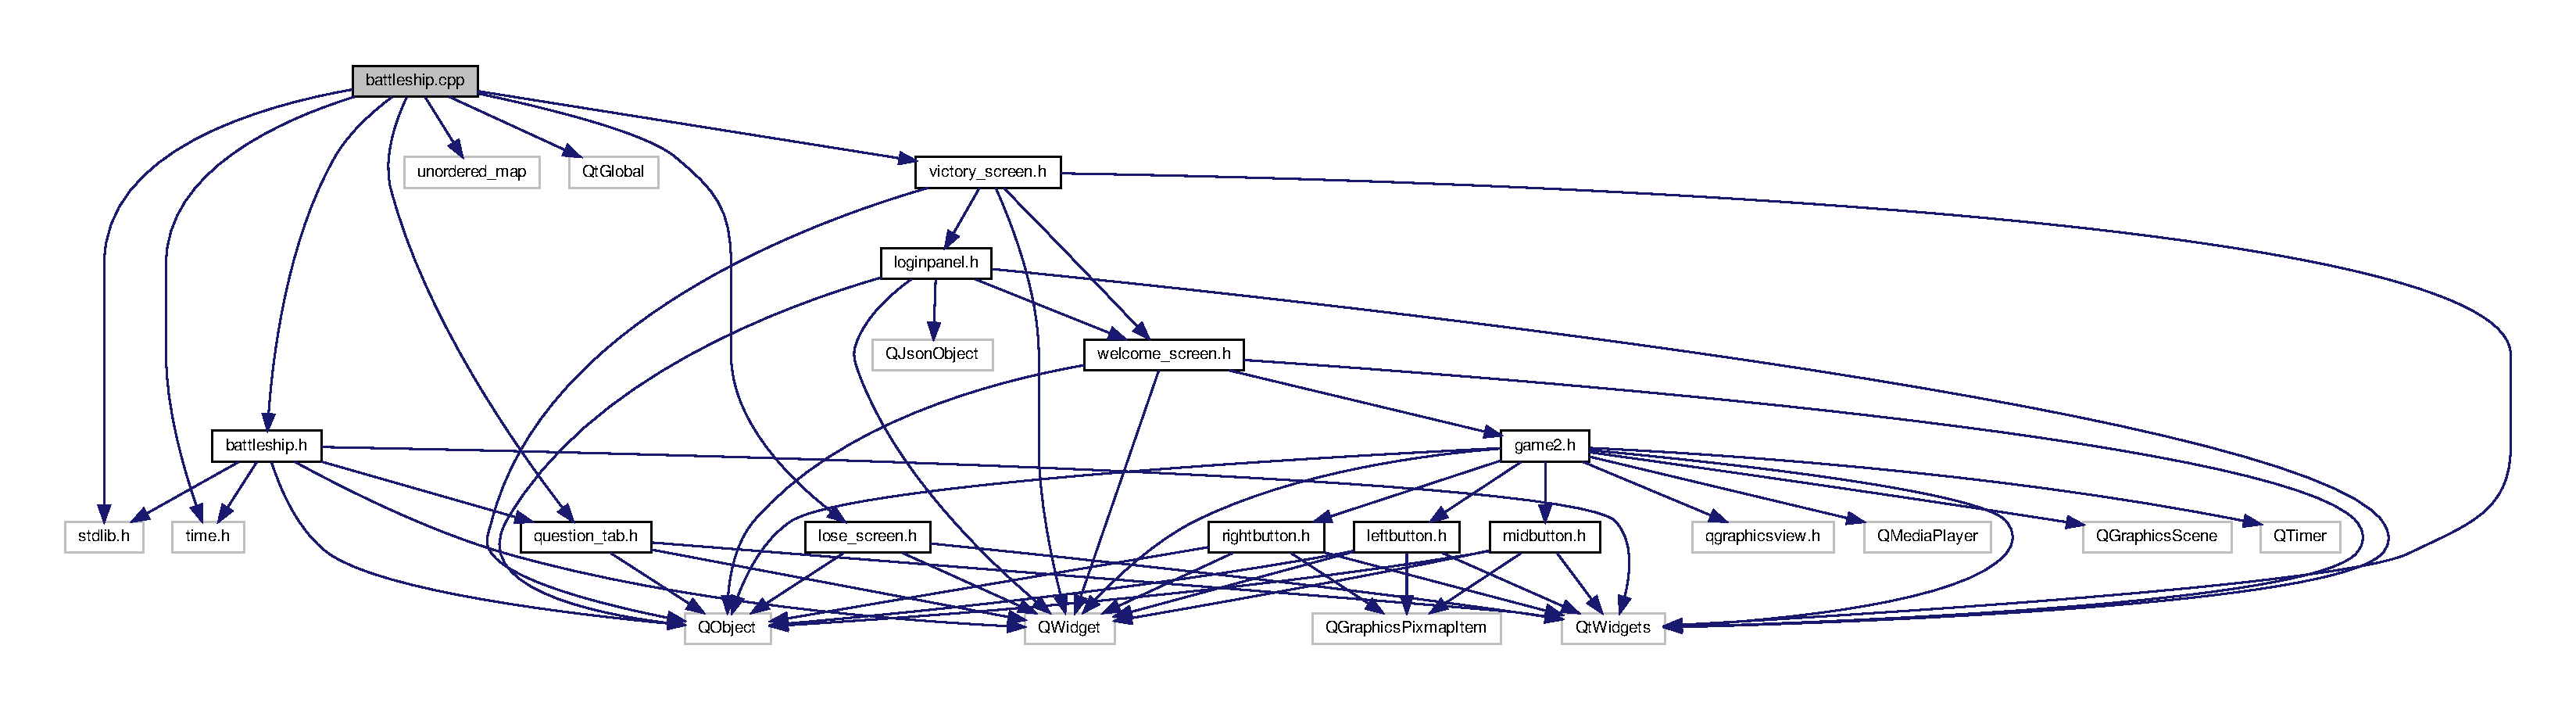
\includegraphics[width=350pt]{battleship_8cpp__incl}
\end{center}
\end{figure}
\subsection*{Macros}
\begin{DoxyCompactItemize}
\item 
\mbox{\Hypertarget{battleship_8cpp_a2c6d8b1b1a798e59c2acfd0a7847c9da}\label{battleship_8cpp_a2c6d8b1b1a798e59c2acfd0a7847c9da}} 
\#define {\bfseries G\+E\+T\+\_\+\+V\+A\+R\+I\+A\+B\+L\+E\+\_\+\+N\+A\+ME}(Variable)~(\#Variable)
\end{DoxyCompactItemize}
\subsection*{Variables}
\begin{DoxyCompactItemize}
\item 
\mbox{\Hypertarget{battleship_8cpp_a77bd4f876bdc3afed5acdd936f775d34}\label{battleship_8cpp_a77bd4f876bdc3afed5acdd936f775d34}} 
int {\bfseries seconds} = 600
\item 
\mbox{\Hypertarget{battleship_8cpp_a94acbe75d9eccc82cdebd3d04aaa3d68}\label{battleship_8cpp_a94acbe75d9eccc82cdebd3d04aaa3d68}} 
int {\bfseries correct} = 0
\item 
\mbox{\Hypertarget{battleship_8cpp_a88ea6d6e114267e884acba52d0464ffe}\label{battleship_8cpp_a88ea6d6e114267e884acba52d0464ffe}} 
int {\bfseries incorrect} = 0
\item 
\mbox{\Hypertarget{battleship_8cpp_ae967c300a67796bafbb974f7324c8461}\label{battleship_8cpp_ae967c300a67796bafbb974f7324c8461}} 
Q\+String {\bfseries question\+\_\+path}
\item 
\mbox{\Hypertarget{battleship_8cpp_a018b0ff0fd0b5684ac437ffc566831f5}\label{battleship_8cpp_a018b0ff0fd0b5684ac437ffc566831f5}} 
Q\+String {\bfseries correct\+\_\+path}
\item 
\mbox{\Hypertarget{battleship_8cpp_acb559820d9ca11295b4500f179ef6392}\label{battleship_8cpp_acb559820d9ca11295b4500f179ef6392}} 
int {\bfseries i} = 0
\item 
\mbox{\Hypertarget{battleship_8cpp_a37d972ae0b47b9099e30983131d31916}\label{battleship_8cpp_a37d972ae0b47b9099e30983131d31916}} 
int {\bfseries j} = -\/1
\item 
\mbox{\Hypertarget{battleship_8cpp_a2474a4788b66890cfb50ccdafdcd8322}\label{battleship_8cpp_a2474a4788b66890cfb50ccdafdcd8322}} 
Q\+List$<$ int $>$ {\bfseries good\+\_\+ships} = Q\+List$<$int$>$\{10,12,13,30,31,32,33\}
\item 
\mbox{\Hypertarget{battleship_8cpp_a9db4b8549c0abf5bd7fa95b22c17823e}\label{battleship_8cpp_a9db4b8549c0abf5bd7fa95b22c17823e}} 
Q\+String {\bfseries path\+\_\+explosion} = \char`\"{}\+:/game1assets/pop.\+png\char`\"{}
\item 
\mbox{\Hypertarget{battleship_8cpp_a5aa1731610537e057191db627c19f1ca}\label{battleship_8cpp_a5aa1731610537e057191db627c19f1ca}} 
int {\bfseries check} = 1
\item 
\mbox{\Hypertarget{battleship_8cpp_af159af6e0bfb9cbe47827ffede96b63d}\label{battleship_8cpp_af159af6e0bfb9cbe47827ffede96b63d}} 
unordered\+\_\+map$<$ string, Q\+String $>$ {\bfseries urlmap}
\item 
\mbox{\Hypertarget{battleship_8cpp_acfbdf8cb47061f51bf94808a1764df19}\label{battleship_8cpp_acfbdf8cb47061f51bf94808a1764df19}} 
unordered\+\_\+map$<$ string, Q\+String $>$ {\bfseries explodedmap}
\end{DoxyCompactItemize}


\subsection{Detailed Description}
battleship 

implementation of battleship class 
\hypertarget{battleship_8h}{}\section{battleship.\+h File Reference}
\label{battleship_8h}\index{battleship.\+h@{battleship.\+h}}


battleship class  


{\ttfamily \#include $<$Q\+Object$>$}\newline
{\ttfamily \#include $<$Q\+Widget$>$}\newline
{\ttfamily \#include $<$Qt\+Widgets$>$}\newline
{\ttfamily \#include $<$stdlib.\+h$>$}\newline
{\ttfamily \#include $<$time.\+h$>$}\newline
{\ttfamily \#include \char`\"{}question\+\_\+tab.\+h\char`\"{}}\newline
Include dependency graph for battleship.\+h\+:\nopagebreak
\begin{figure}[H]
\begin{center}
\leavevmode
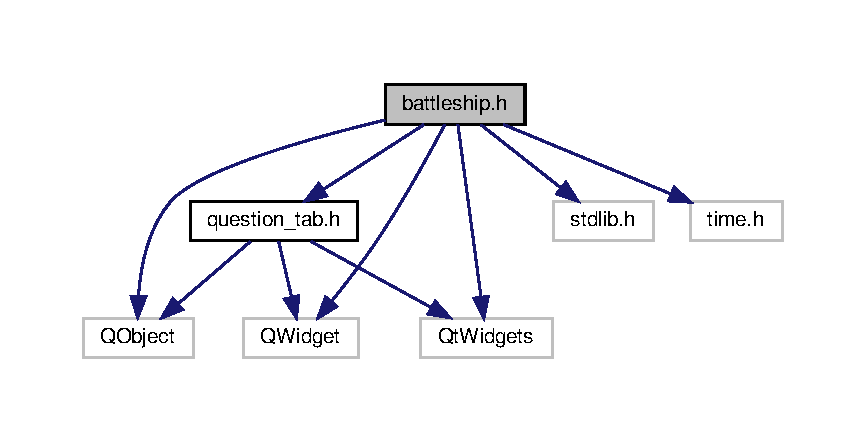
\includegraphics[width=350pt]{battleship_8h__incl}
\end{center}
\end{figure}
This graph shows which files directly or indirectly include this file\+:\nopagebreak
\begin{figure}[H]
\begin{center}
\leavevmode
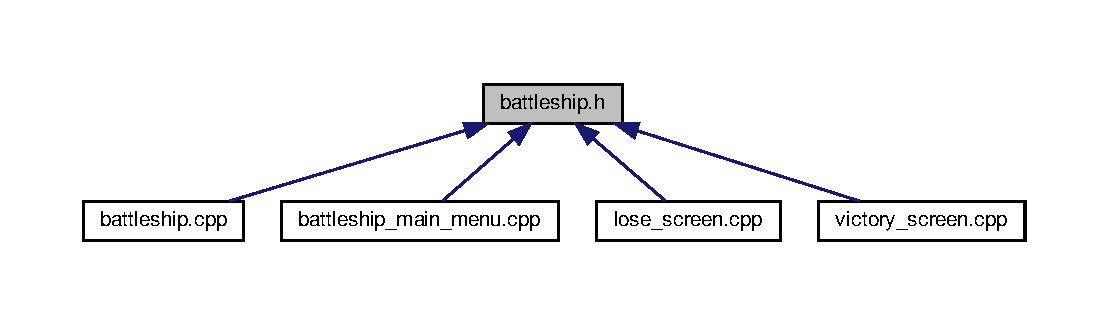
\includegraphics[width=350pt]{battleship_8h__dep__incl}
\end{center}
\end{figure}
\subsection*{Classes}
\begin{DoxyCompactItemize}
\item 
class \hyperlink{classbattleship}{battleship}
\end{DoxyCompactItemize}


\subsection{Detailed Description}
battleship class 

class responsible for the battleship game 
\hypertarget{battleship__main__menu_8cpp}{}\section{battleship\+\_\+main\+\_\+menu.\+cpp File Reference}
\label{battleship__main__menu_8cpp}\index{battleship\+\_\+main\+\_\+menu.\+cpp@{battleship\+\_\+main\+\_\+menu.\+cpp}}


battleship main menu  


{\ttfamily \#include \char`\"{}battleship\+\_\+main\+\_\+menu.\+h\char`\"{}}\newline
{\ttfamily \#include \char`\"{}battleship.\+h\char`\"{}}\newline
{\ttfamily \#include $<$iostream$>$}\newline
Include dependency graph for battleship\+\_\+main\+\_\+menu.\+cpp\+:\nopagebreak
\begin{figure}[H]
\begin{center}
\leavevmode
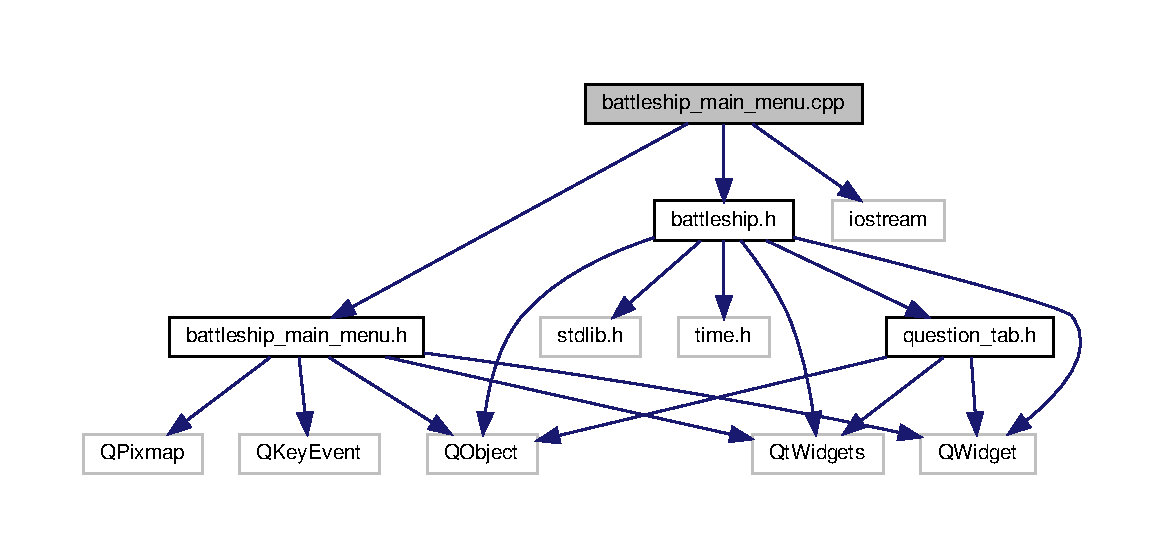
\includegraphics[width=350pt]{battleship__main__menu_8cpp__incl}
\end{center}
\end{figure}


\subsection{Detailed Description}
battleship main menu 

implementation of battleship main menu class 
\hypertarget{battleship__main__menu_8h}{}\section{battleship\+\_\+main\+\_\+menu.\+h File Reference}
\label{battleship__main__menu_8h}\index{battleship\+\_\+main\+\_\+menu.\+h@{battleship\+\_\+main\+\_\+menu.\+h}}


battleship main menu class  


{\ttfamily \#include $<$Q\+Object$>$}\newline
{\ttfamily \#include $<$Q\+Widget$>$}\newline
{\ttfamily \#include $<$Qt\+Widgets$>$}\newline
{\ttfamily \#include $<$Q\+Pixmap$>$}\newline
{\ttfamily \#include $<$Q\+Key\+Event$>$}\newline
Include dependency graph for battleship\+\_\+main\+\_\+menu.\+h\+:\nopagebreak
\begin{figure}[H]
\begin{center}
\leavevmode
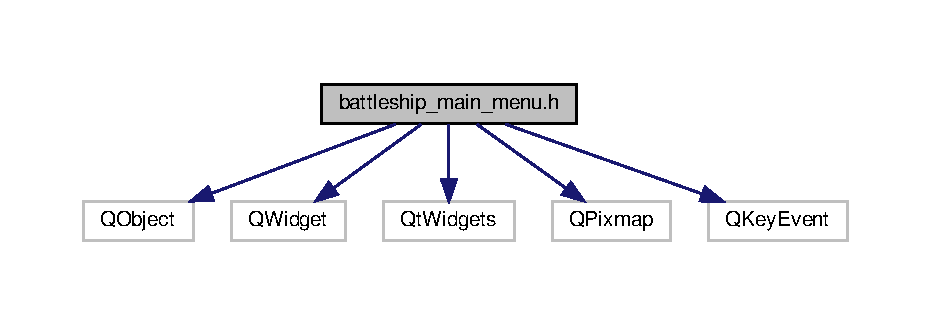
\includegraphics[width=350pt]{battleship__main__menu_8h__incl}
\end{center}
\end{figure}
This graph shows which files directly or indirectly include this file\+:\nopagebreak
\begin{figure}[H]
\begin{center}
\leavevmode
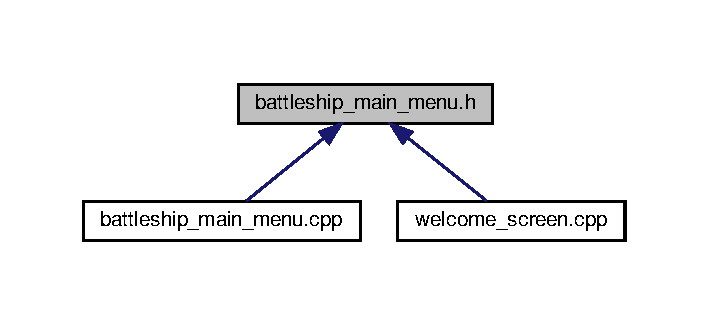
\includegraphics[width=340pt]{battleship__main__menu_8h__dep__incl}
\end{center}
\end{figure}
\subsection*{Classes}
\begin{DoxyCompactItemize}
\item 
class \hyperlink{classBattleship__Main__Menu}{Battleship\+\_\+\+Main\+\_\+\+Menu}
\end{DoxyCompactItemize}


\subsection{Detailed Description}
battleship main menu class 

class responsible for setting up the main menu of the battleship game 
\hypertarget{extern__vars_8h}{}\section{extern\+\_\+vars.\+h File Reference}
\label{extern__vars_8h}\index{extern\+\_\+vars.\+h@{extern\+\_\+vars.\+h}}


extern\+\_\+vars class  


{\ttfamily \#include $<$qgraphicsview.\+h$>$}\newline
{\ttfamily \#include \char`\"{}game2.\+h\char`\"{}}\newline
Include dependency graph for extern\+\_\+vars.\+h\+:\nopagebreak
\begin{figure}[H]
\begin{center}
\leavevmode
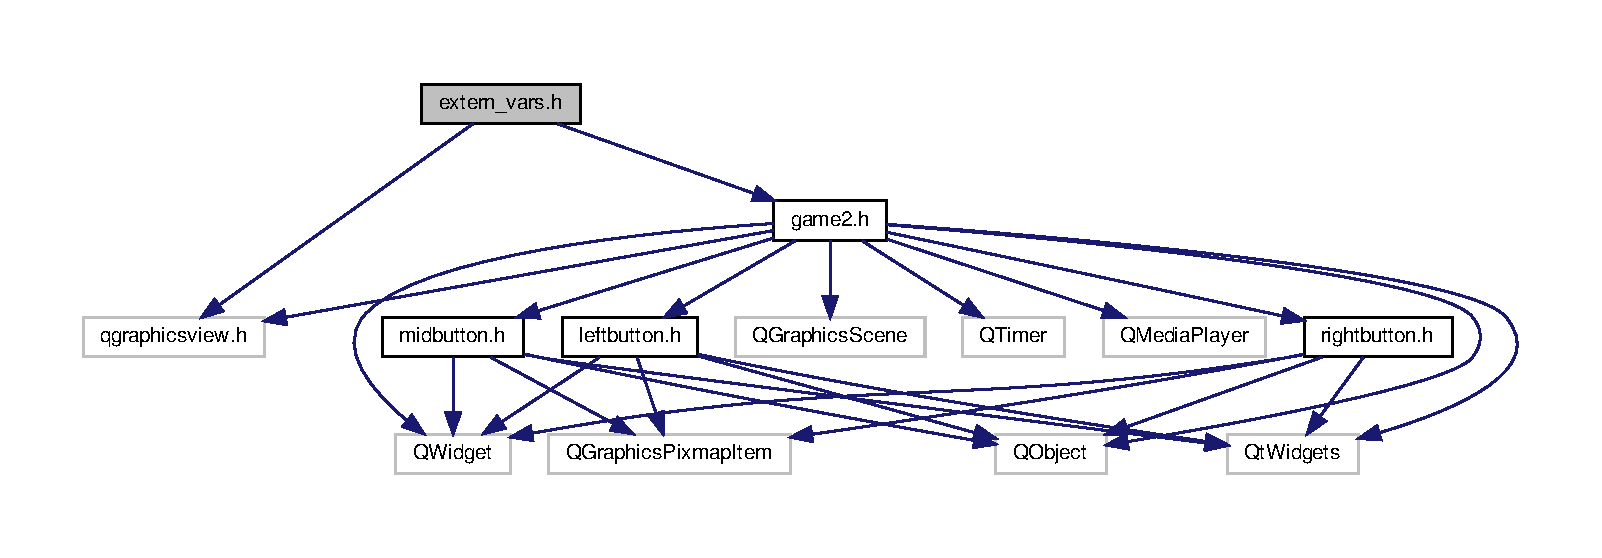
\includegraphics[width=350pt]{extern__vars_8h__incl}
\end{center}
\end{figure}
This graph shows which files directly or indirectly include this file\+:\nopagebreak
\begin{figure}[H]
\begin{center}
\leavevmode
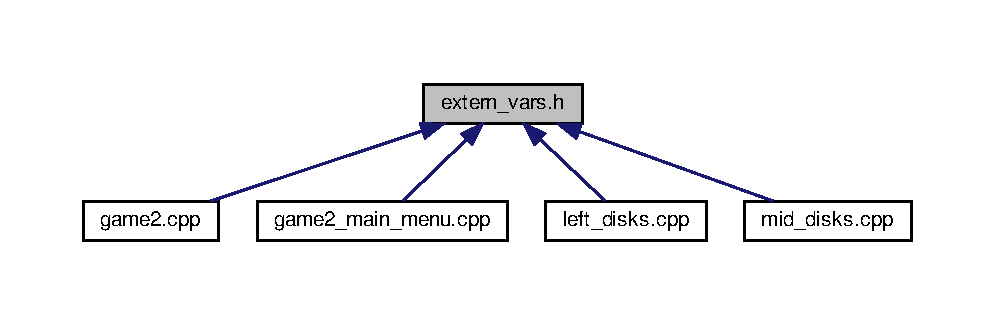
\includegraphics[width=350pt]{extern__vars_8h__dep__incl}
\end{center}
\end{figure}
\subsection*{Variables}
\begin{DoxyCompactItemize}
\item 
int \hyperlink{extern__vars_8h_a6326921112efa5d8d46fa16601d07a9d}{missed\+\_\+disks}
\begin{DoxyCompactList}\small\item\em Counter for missed discs. \end{DoxyCompactList}\item 
int \hyperlink{extern__vars_8h_ad5255b2ed36beca0ba85eda17d99c421}{total\+\_\+score}
\begin{DoxyCompactList}\small\item\em Counter for total score. \end{DoxyCompactList}\item 
\mbox{\Hypertarget{extern__vars_8h_adce1d2607dd60b86675eb9a624adb3de}\label{extern__vars_8h_adce1d2607dd60b86675eb9a624adb3de}} 
Q\+String \hyperlink{extern__vars_8h_adce1d2607dd60b86675eb9a624adb3de}{ans}
\begin{DoxyCompactList}\small\item\em Choice of difficulty. \end{DoxyCompactList}\end{DoxyCompactItemize}


\subsection{Detailed Description}
extern\+\_\+vars class 

class that contains external global variables to be used across different files 

\subsection{Variable Documentation}
\mbox{\Hypertarget{extern__vars_8h_a6326921112efa5d8d46fa16601d07a9d}\label{extern__vars_8h_a6326921112efa5d8d46fa16601d07a9d}} 
\index{extern\+\_\+vars.\+h@{extern\+\_\+vars.\+h}!missed\+\_\+disks@{missed\+\_\+disks}}
\index{missed\+\_\+disks@{missed\+\_\+disks}!extern\+\_\+vars.\+h@{extern\+\_\+vars.\+h}}
\subsubsection{\texorpdfstring{missed\+\_\+disks}{missed\_disks}}
{\footnotesize\ttfamily int missed\+\_\+disks}



Counter for missed discs. 

Counter for missed discs. \mbox{\Hypertarget{extern__vars_8h_ad5255b2ed36beca0ba85eda17d99c421}\label{extern__vars_8h_ad5255b2ed36beca0ba85eda17d99c421}} 
\index{extern\+\_\+vars.\+h@{extern\+\_\+vars.\+h}!total\+\_\+score@{total\+\_\+score}}
\index{total\+\_\+score@{total\+\_\+score}!extern\+\_\+vars.\+h@{extern\+\_\+vars.\+h}}
\subsubsection{\texorpdfstring{total\+\_\+score}{total\_score}}
{\footnotesize\ttfamily int total\+\_\+score}



Counter for total score. 

Counter for total score. 
\hypertarget{game2_8cpp}{}\section{game2.\+cpp File Reference}
\label{game2_8cpp}\index{game2.\+cpp@{game2.\+cpp}}


\hyperlink{classgame2}{game2}  


{\ttfamily \#include \char`\"{}game2.\+h\char`\"{}}\newline
{\ttfamily \#include \char`\"{}left\+\_\+disks.\+h\char`\"{}}\newline
{\ttfamily \#include \char`\"{}mid\+\_\+disks.\+h\char`\"{}}\newline
{\ttfamily \#include \char`\"{}right\+\_\+disks.\+h\char`\"{}}\newline
{\ttfamily \#include \char`\"{}welcome\+\_\+screen.\+h\char`\"{}}\newline
{\ttfamily \#include $<$Q\+Object$>$}\newline
{\ttfamily \#include $<$Q\+Widget$>$}\newline
{\ttfamily \#include $<$Q\+Debug$>$}\newline
{\ttfamily \#include $<$Q\+Graphics\+Pixmap\+Item$>$}\newline
{\ttfamily \#include $<$Q\+Timer$>$}\newline
{\ttfamily \#include $<$Q\+Graphics\+Path\+Item$>$}\newline
{\ttfamily \#include \char`\"{}victory\+\_\+screen.\+h\char`\"{}}\newline
{\ttfamily \#include \char`\"{}lose\+\_\+screen.\+h\char`\"{}}\newline
{\ttfamily \#include \char`\"{}extern\+\_\+vars.\+h\char`\"{}}\newline
{\ttfamily \#include $<$Q\+Media\+Playlist$>$}\newline
Include dependency graph for game2.\+cpp\+:\nopagebreak
\begin{figure}[H]
\begin{center}
\leavevmode
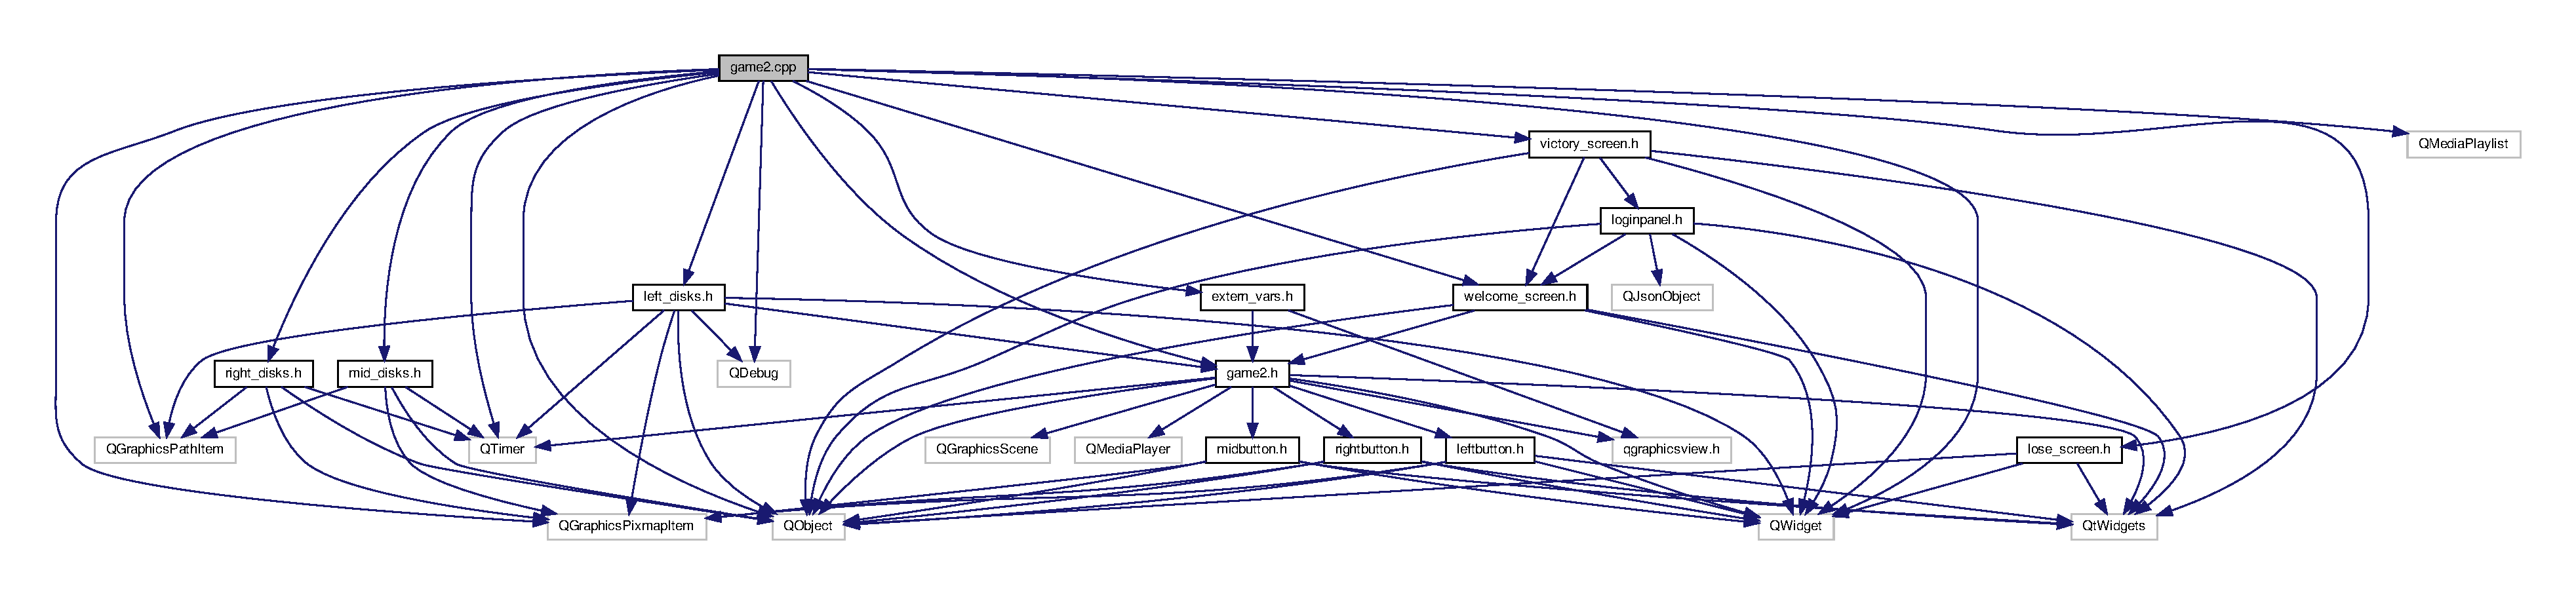
\includegraphics[width=350pt]{game2_8cpp__incl}
\end{center}
\end{figure}
\subsection*{Variables}
\begin{DoxyCompactItemize}
\item 
\mbox{\Hypertarget{game2_8cpp_a92e4453fad760c994eea1323e52198dd}\label{game2_8cpp_a92e4453fad760c994eea1323e52198dd}} 
int \hyperlink{game2_8cpp_a92e4453fad760c994eea1323e52198dd}{counter\+\_\+red} = 0
\begin{DoxyCompactList}\small\item\em Counter for red discs. \end{DoxyCompactList}\item 
\mbox{\Hypertarget{game2_8cpp_abc2f9d7acffb04e74b5f18cbc82c1427}\label{game2_8cpp_abc2f9d7acffb04e74b5f18cbc82c1427}} 
int \hyperlink{game2_8cpp_abc2f9d7acffb04e74b5f18cbc82c1427}{counter\+\_\+yellow} = 0
\begin{DoxyCompactList}\small\item\em Counter for yellow discs. \end{DoxyCompactList}\item 
\mbox{\Hypertarget{game2_8cpp_a19927408ccf3e4db3a4b2c83861fdbfe}\label{game2_8cpp_a19927408ccf3e4db3a4b2c83861fdbfe}} 
int \hyperlink{game2_8cpp_a19927408ccf3e4db3a4b2c83861fdbfe}{counter\+\_\+blue} = 0
\begin{DoxyCompactList}\small\item\em Counter for blue discs. \end{DoxyCompactList}\item 
int \hyperlink{game2_8cpp_ad5255b2ed36beca0ba85eda17d99c421}{total\+\_\+score} = 0
\begin{DoxyCompactList}\small\item\em Total score counter. \end{DoxyCompactList}\item 
int \hyperlink{game2_8cpp_a6326921112efa5d8d46fa16601d07a9d}{missed\+\_\+disks} = 0
\begin{DoxyCompactList}\small\item\em Missed discs counter. \end{DoxyCompactList}\item 
\mbox{\Hypertarget{game2_8cpp_a9a2b31e1552f96a1e64749f49e11d914}\label{game2_8cpp_a9a2b31e1552f96a1e64749f49e11d914}} 
Q\+Timer $\ast$ \hyperlink{game2_8cpp_a9a2b31e1552f96a1e64749f49e11d914}{timer\+\_\+left} = new Q\+Timer()
\begin{DoxyCompactList}\small\item\em Timer for spawning left discs on easy mode. \end{DoxyCompactList}\item 
\mbox{\Hypertarget{game2_8cpp_ab29ef84a56600612c85e13d4ab8ac361}\label{game2_8cpp_ab29ef84a56600612c85e13d4ab8ac361}} 
Q\+Timer $\ast$ \hyperlink{game2_8cpp_ab29ef84a56600612c85e13d4ab8ac361}{timer\+\_\+mid} = new Q\+Timer()
\begin{DoxyCompactList}\small\item\em Timer for spawning middle discs on easy mode. \end{DoxyCompactList}\item 
\mbox{\Hypertarget{game2_8cpp_a2313e67ce1d752d90f657baa0c1616b3}\label{game2_8cpp_a2313e67ce1d752d90f657baa0c1616b3}} 
Q\+Timer $\ast$ \hyperlink{game2_8cpp_a2313e67ce1d752d90f657baa0c1616b3}{timer\+\_\+right} = new Q\+Timer()
\begin{DoxyCompactList}\small\item\em Timer for spawning right discs on easy mode. \end{DoxyCompactList}\item 
\mbox{\Hypertarget{game2_8cpp_a3bec066694e0433031cb7dd8c1a013ac}\label{game2_8cpp_a3bec066694e0433031cb7dd8c1a013ac}} 
Q\+Timer $\ast$ \hyperlink{game2_8cpp_a3bec066694e0433031cb7dd8c1a013ac}{timer\+\_\+left\+\_\+medium} = new Q\+Timer()
\begin{DoxyCompactList}\small\item\em Timer for spawning left discs on medium mode. \end{DoxyCompactList}\item 
\mbox{\Hypertarget{game2_8cpp_a7b4c6b7e50b60d7880ea492b3dbf0dd1}\label{game2_8cpp_a7b4c6b7e50b60d7880ea492b3dbf0dd1}} 
Q\+Timer $\ast$ \hyperlink{game2_8cpp_a7b4c6b7e50b60d7880ea492b3dbf0dd1}{timer\+\_\+mid\+\_\+medium} = new Q\+Timer()
\begin{DoxyCompactList}\small\item\em Timer for spawning middle discs on medium mode. \end{DoxyCompactList}\item 
\mbox{\Hypertarget{game2_8cpp_a26286620e13aee0d06462d819c0f8f29}\label{game2_8cpp_a26286620e13aee0d06462d819c0f8f29}} 
Q\+Timer $\ast$ \hyperlink{game2_8cpp_a26286620e13aee0d06462d819c0f8f29}{timer\+\_\+right\+\_\+medium} = new Q\+Timer()
\begin{DoxyCompactList}\small\item\em Timer for spawning right dics on medium mode. \end{DoxyCompactList}\item 
\mbox{\Hypertarget{game2_8cpp_ac0c40e8e87c07fbd3998ac9fdde9e899}\label{game2_8cpp_ac0c40e8e87c07fbd3998ac9fdde9e899}} 
Q\+Timer $\ast$ \hyperlink{game2_8cpp_ac0c40e8e87c07fbd3998ac9fdde9e899}{timer\+\_\+left\+\_\+hard} = new Q\+Timer()
\begin{DoxyCompactList}\small\item\em Timer for spawning left discs on hard mode. \end{DoxyCompactList}\item 
\mbox{\Hypertarget{game2_8cpp_a173161b2b864495223375038827d9169}\label{game2_8cpp_a173161b2b864495223375038827d9169}} 
Q\+Timer $\ast$ \hyperlink{game2_8cpp_a173161b2b864495223375038827d9169}{timer\+\_\+mid\+\_\+hard} = new Q\+Timer()
\begin{DoxyCompactList}\small\item\em Timer for spawning middle discs on hard mode. \end{DoxyCompactList}\item 
\mbox{\Hypertarget{game2_8cpp_abd3605eb182cbb316c545b97a6ed9d93}\label{game2_8cpp_abd3605eb182cbb316c545b97a6ed9d93}} 
Q\+Timer $\ast$ \hyperlink{game2_8cpp_abd3605eb182cbb316c545b97a6ed9d93}{timer\+\_\+right\+\_\+hard} = new Q\+Timer()
\begin{DoxyCompactList}\small\item\em Timer for spawning right discs on hard mode. \end{DoxyCompactList}\item 
\mbox{\Hypertarget{game2_8cpp_a13c0073e5a590ed3716b8eba94e646b3}\label{game2_8cpp_a13c0073e5a590ed3716b8eba94e646b3}} 
Q\+Media\+Playlist $\ast$ {\bfseries playlist} = new Q\+Media\+Playlist()
\item 
\mbox{\Hypertarget{game2_8cpp_aed53840f09606a90ee24365ffec548c8}\label{game2_8cpp_aed53840f09606a90ee24365ffec548c8}} 
Q\+Media\+Player $\ast$ \hyperlink{game2_8cpp_aed53840f09606a90ee24365ffec548c8}{music} = new Q\+Media\+Player()
\begin{DoxyCompactList}\small\item\em For game music. \end{DoxyCompactList}\end{DoxyCompactItemize}


\subsection{Detailed Description}
\hyperlink{classgame2}{game2} 

implementation of \hyperlink{classgame2}{game2} class 

\subsection{Variable Documentation}
\mbox{\Hypertarget{game2_8cpp_a6326921112efa5d8d46fa16601d07a9d}\label{game2_8cpp_a6326921112efa5d8d46fa16601d07a9d}} 
\index{game2.\+cpp@{game2.\+cpp}!missed\+\_\+disks@{missed\+\_\+disks}}
\index{missed\+\_\+disks@{missed\+\_\+disks}!game2.\+cpp@{game2.\+cpp}}
\subsubsection{\texorpdfstring{missed\+\_\+disks}{missed\_disks}}
{\footnotesize\ttfamily int missed\+\_\+disks = 0}



Missed discs counter. 

Counter for missed discs. \mbox{\Hypertarget{game2_8cpp_ad5255b2ed36beca0ba85eda17d99c421}\label{game2_8cpp_ad5255b2ed36beca0ba85eda17d99c421}} 
\index{game2.\+cpp@{game2.\+cpp}!total\+\_\+score@{total\+\_\+score}}
\index{total\+\_\+score@{total\+\_\+score}!game2.\+cpp@{game2.\+cpp}}
\subsubsection{\texorpdfstring{total\+\_\+score}{total\_score}}
{\footnotesize\ttfamily int total\+\_\+score = 0}



Total score counter. 

Counter for total score. 
\hypertarget{game2_8h}{}\section{game2.\+h File Reference}
\label{game2_8h}\index{game2.\+h@{game2.\+h}}


\hyperlink{classgame2}{game2} class  


{\ttfamily \#include $<$Q\+Object$>$}\newline
{\ttfamily \#include $<$Q\+Widget$>$}\newline
{\ttfamily \#include $<$Qt\+Widgets$>$}\newline
{\ttfamily \#include $<$Q\+Graphics\+Scene$>$}\newline
{\ttfamily \#include $<$Q\+Timer$>$}\newline
{\ttfamily \#include \char`\"{}leftbutton.\+h\char`\"{}}\newline
{\ttfamily \#include \char`\"{}midbutton.\+h\char`\"{}}\newline
{\ttfamily \#include \char`\"{}rightbutton.\+h\char`\"{}}\newline
{\ttfamily \#include \char`\"{}qgraphicsview.\+h\char`\"{}}\newline
{\ttfamily \#include $<$Q\+Media\+Player$>$}\newline
Include dependency graph for game2.\+h\+:\nopagebreak
\begin{figure}[H]
\begin{center}
\leavevmode
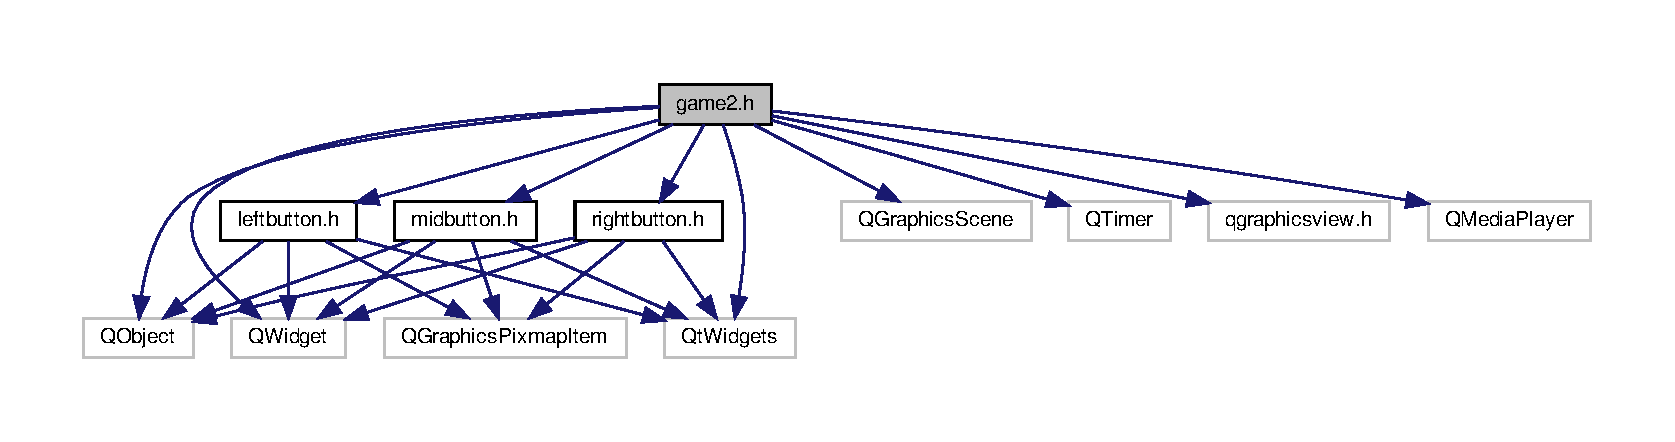
\includegraphics[width=350pt]{game2_8h__incl}
\end{center}
\end{figure}
This graph shows which files directly or indirectly include this file\+:\nopagebreak
\begin{figure}[H]
\begin{center}
\leavevmode
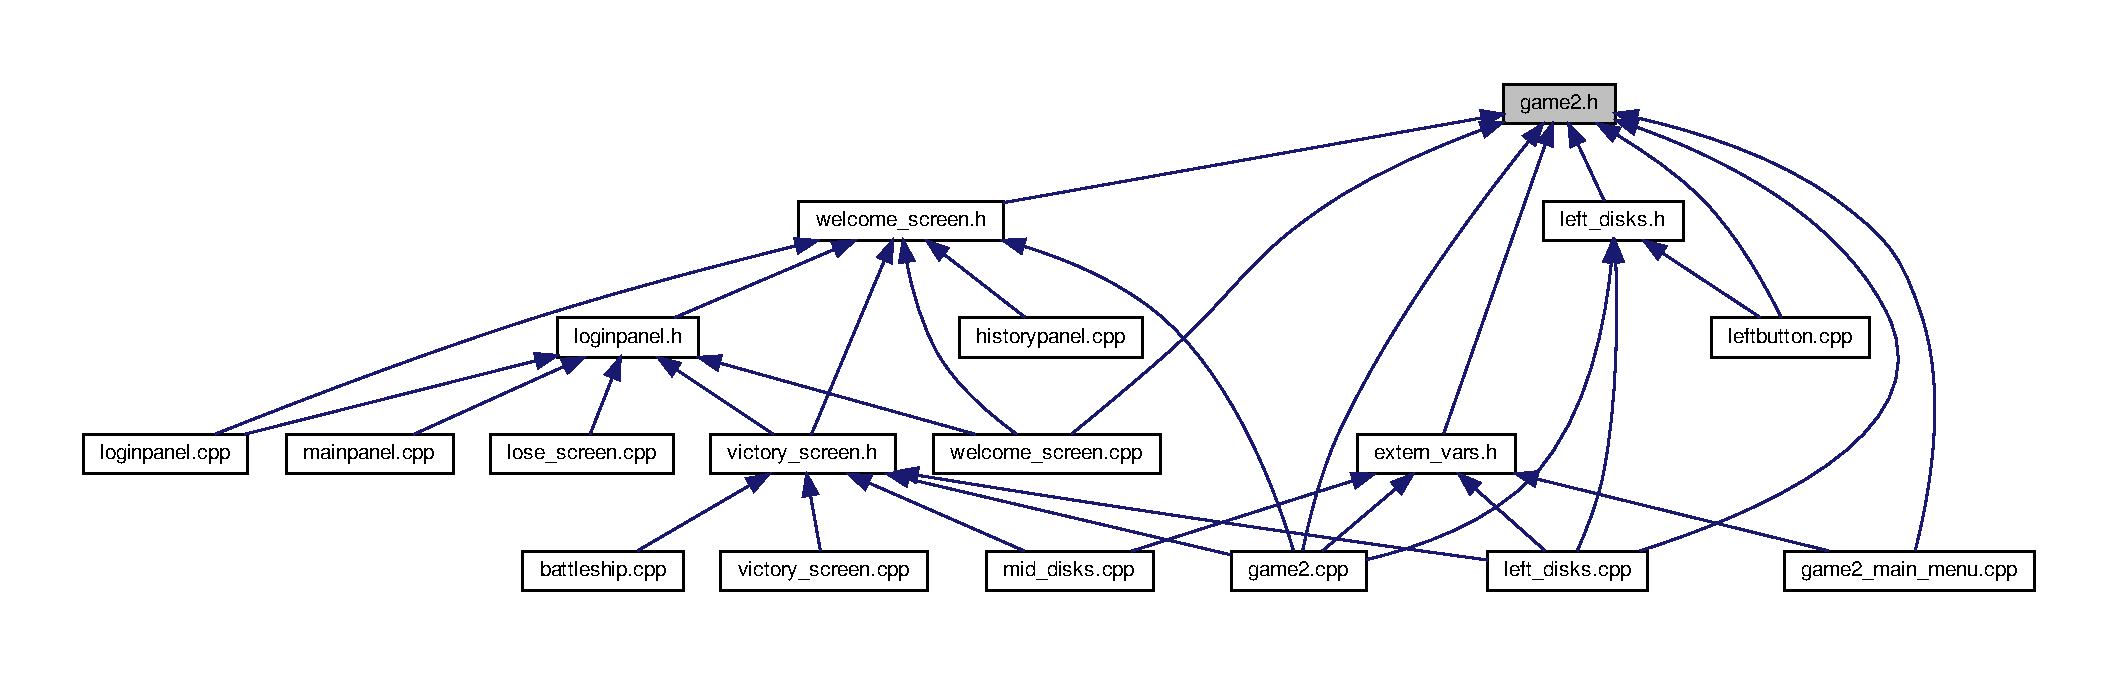
\includegraphics[width=350pt]{game2_8h__dep__incl}
\end{center}
\end{figure}
\subsection*{Classes}
\begin{DoxyCompactItemize}
\item 
class \hyperlink{classgame2}{game2}
\end{DoxyCompactItemize}


\subsection{Detailed Description}
\hyperlink{classgame2}{game2} class 

class responsible for the shooting discs game 
\hypertarget{game2__main__menu_8cpp}{}\section{game2\+\_\+main\+\_\+menu.\+cpp File Reference}
\label{game2__main__menu_8cpp}\index{game2\+\_\+main\+\_\+menu.\+cpp@{game2\+\_\+main\+\_\+menu.\+cpp}}


\hyperlink{classgame2}{game2} main menu  


{\ttfamily \#include \char`\"{}game2\+\_\+main\+\_\+menu.\+h\char`\"{}}\newline
{\ttfamily \#include \char`\"{}game2.\+h\char`\"{}}\newline
{\ttfamily \#include \char`\"{}extern\+\_\+vars.\+h\char`\"{}}\newline
Include dependency graph for game2\+\_\+main\+\_\+menu.\+cpp\+:\nopagebreak
\begin{figure}[H]
\begin{center}
\leavevmode
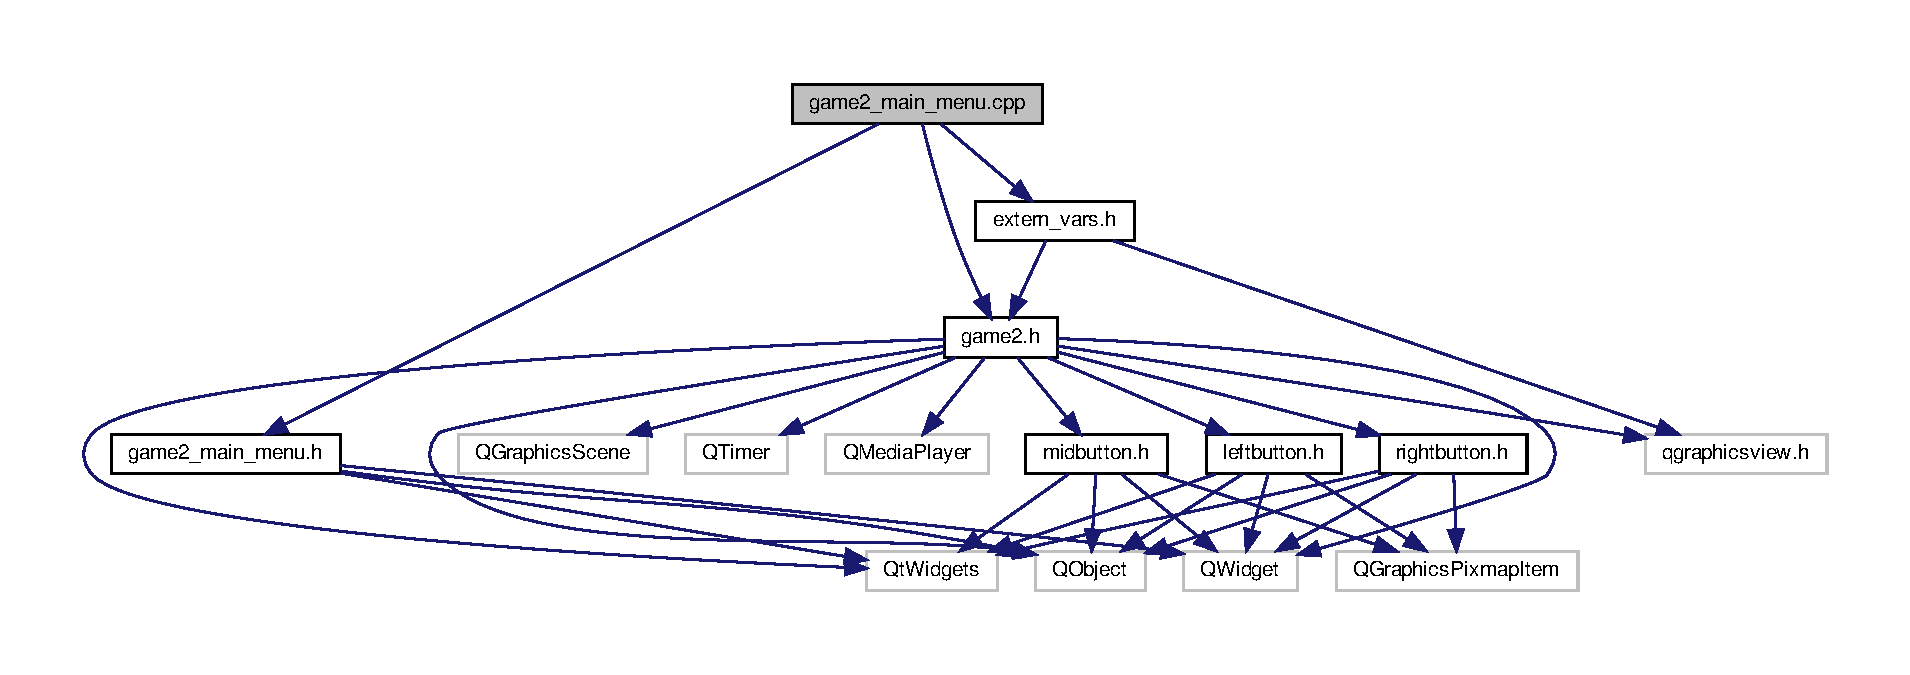
\includegraphics[width=350pt]{game2__main__menu_8cpp__incl}
\end{center}
\end{figure}
\subsection*{Variables}
\begin{DoxyCompactItemize}
\item 
\mbox{\Hypertarget{game2__main__menu_8cpp_adce1d2607dd60b86675eb9a624adb3de}\label{game2__main__menu_8cpp_adce1d2607dd60b86675eb9a624adb3de}} 
Q\+String \hyperlink{game2__main__menu_8cpp_adce1d2607dd60b86675eb9a624adb3de}{ans} = \char`\"{}\char`\"{}
\begin{DoxyCompactList}\small\item\em Choice of difficulty. \end{DoxyCompactList}\end{DoxyCompactItemize}


\subsection{Detailed Description}
\hyperlink{classgame2}{game2} main menu 

implementation of \hyperlink{classgame2}{game2} main menu class 
\hypertarget{game2__main__menu_8h}{}\section{game2\+\_\+main\+\_\+menu.\+h File Reference}
\label{game2__main__menu_8h}\index{game2\+\_\+main\+\_\+menu.\+h@{game2\+\_\+main\+\_\+menu.\+h}}


\hyperlink{classgame2}{game2} main meenu class  


{\ttfamily \#include $<$Q\+Object$>$}\newline
{\ttfamily \#include $<$Q\+Widget$>$}\newline
{\ttfamily \#include $<$Qt\+Widgets$>$}\newline
Include dependency graph for game2\+\_\+main\+\_\+menu.\+h\+:\nopagebreak
\begin{figure}[H]
\begin{center}
\leavevmode
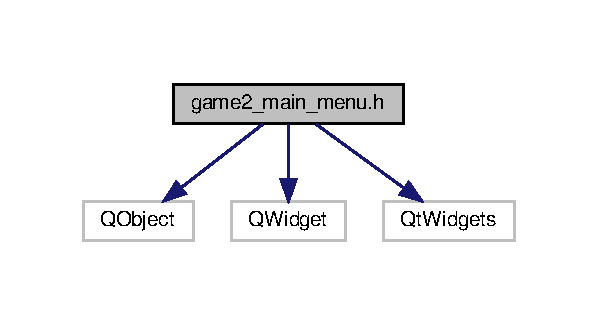
\includegraphics[width=287pt]{game2__main__menu_8h__incl}
\end{center}
\end{figure}
This graph shows which files directly or indirectly include this file\+:\nopagebreak
\begin{figure}[H]
\begin{center}
\leavevmode
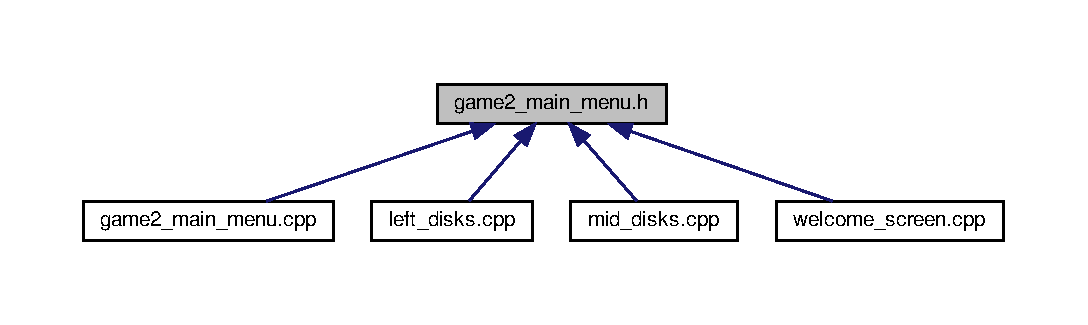
\includegraphics[width=350pt]{game2__main__menu_8h__dep__incl}
\end{center}
\end{figure}
\subsection*{Classes}
\begin{DoxyCompactItemize}
\item 
class \hyperlink{classgame2__main__menu}{game2\+\_\+main\+\_\+menu}
\end{DoxyCompactItemize}


\subsection{Detailed Description}
\hyperlink{classgame2}{game2} main meenu class 

class responsible for the shooting discs game 
\hypertarget{historypanel_8cpp}{}\section{historypanel.\+cpp File Reference}
\label{historypanel_8cpp}\index{historypanel.\+cpp@{historypanel.\+cpp}}


user game history implementation  


{\ttfamily \#include \char`\"{}historypanel.\+h\char`\"{}}\newline
{\ttfamily \#include \char`\"{}welcome\+\_\+screen.\+h\char`\"{}}\newline
Include dependency graph for historypanel.\+cpp\+:\nopagebreak
\begin{figure}[H]
\begin{center}
\leavevmode
\includegraphics[width=350pt]{historypanel_8cpp__incl}
\end{center}
\end{figure}


\subsection{Detailed Description}
user game history implementation 


\hypertarget{historypanel_8h}{}\section{historypanel.\+h File Reference}
\label{historypanel_8h}\index{historypanel.\+h@{historypanel.\+h}}


user game history  


{\ttfamily \#include $<$Q\+Object$>$}\newline
{\ttfamily \#include $<$Q\+Widget$>$}\newline
{\ttfamily \#include $<$Qt\+Widgets$>$}\newline
{\ttfamily \#include $<$Q\+Json\+Object$>$}\newline
Include dependency graph for historypanel.\+h\+:\nopagebreak
\begin{figure}[H]
\begin{center}
\leavevmode
\includegraphics[width=350pt]{historypanel_8h__incl}
\end{center}
\end{figure}
This graph shows which files directly or indirectly include this file\+:\nopagebreak
\begin{figure}[H]
\begin{center}
\leavevmode
\includegraphics[width=296pt]{historypanel_8h__dep__incl}
\end{center}
\end{figure}
\subsection*{Classes}
\begin{DoxyCompactItemize}
\item 
class \hyperlink{classhistorypanel}{historypanel}
\end{DoxyCompactItemize}


\subsection{Detailed Description}
user game history 


\hypertarget{left__disks_8cpp}{}\section{left\+\_\+disks.\+cpp File Reference}
\label{left__disks_8cpp}\index{left\+\_\+disks.\+cpp@{left\+\_\+disks.\+cpp}}


left discs  


{\ttfamily \#include \char`\"{}left\+\_\+disks.\+h\char`\"{}}\newline
{\ttfamily \#include $<$qgraphicsscene.\+h$>$}\newline
{\ttfamily \#include $<$Q\+Key\+Event$>$}\newline
{\ttfamily \#include $<$Q\+Point$>$}\newline
{\ttfamily \#include $<$iostream$>$}\newline
{\ttfamily \#include \char`\"{}extern\+\_\+vars.\+h\char`\"{}}\newline
{\ttfamily \#include \char`\"{}lose\+\_\+screen.\+h\char`\"{}}\newline
{\ttfamily \#include \char`\"{}victory\+\_\+screen.\+h\char`\"{}}\newline
{\ttfamily \#include \char`\"{}game2\+\_\+main\+\_\+menu.\+h\char`\"{}}\newline
{\ttfamily \#include \char`\"{}game2.\+h\char`\"{}}\newline
Include dependency graph for left\+\_\+disks.\+cpp\+:\nopagebreak
\begin{figure}[H]
\begin{center}
\leavevmode
\includegraphics[width=350pt]{left__disks_8cpp__incl}
\end{center}
\end{figure}


\subsection{Detailed Description}
left discs 

implementation of the \hyperlink{classleft__disks}{left\+\_\+disks} class 
\hypertarget{left__disks_8h}{}\section{left\+\_\+disks.\+h File Reference}
\label{left__disks_8h}\index{left\+\_\+disks.\+h@{left\+\_\+disks.\+h}}


left discs class  


{\ttfamily \#include \char`\"{}game2.\+h\char`\"{}}\newline
{\ttfamily \#include $<$Q\+Object$>$}\newline
{\ttfamily \#include $<$Q\+Widget$>$}\newline
{\ttfamily \#include $<$Q\+Debug$>$}\newline
{\ttfamily \#include $<$Q\+Graphics\+Pixmap\+Item$>$}\newline
{\ttfamily \#include $<$Q\+Timer$>$}\newline
{\ttfamily \#include $<$Q\+Graphics\+Path\+Item$>$}\newline
Include dependency graph for left\+\_\+disks.\+h\+:\nopagebreak
\begin{figure}[H]
\begin{center}
\leavevmode
\includegraphics[width=350pt]{left__disks_8h__incl}
\end{center}
\end{figure}
This graph shows which files directly or indirectly include this file\+:\nopagebreak
\begin{figure}[H]
\begin{center}
\leavevmode
\includegraphics[width=335pt]{left__disks_8h__dep__incl}
\end{center}
\end{figure}
\subsection*{Classes}
\begin{DoxyCompactItemize}
\item 
class \hyperlink{classleft__disks}{left\+\_\+disks}
\end{DoxyCompactItemize}


\subsection{Detailed Description}
left discs class 

class responsible for handling left discs 
\hypertarget{leftbutton_8cpp}{}\section{leftbutton.\+cpp File Reference}
\label{leftbutton_8cpp}\index{leftbutton.\+cpp@{leftbutton.\+cpp}}


leftbutton  


{\ttfamily \#include \char`\"{}leftbutton.\+h\char`\"{}}\newline
{\ttfamily \#include \char`\"{}left\+\_\+disks.\+h\char`\"{}}\newline
{\ttfamily \#include \char`\"{}game2.\+h\char`\"{}}\newline
Include dependency graph for leftbutton.\+cpp\+:\nopagebreak
\begin{figure}[H]
\begin{center}
\leavevmode
\includegraphics[width=350pt]{leftbutton_8cpp__incl}
\end{center}
\end{figure}


\subsection{Detailed Description}
leftbutton 

implementation of leftbutton class 
\hypertarget{leftbutton_8h}{}\section{leftbutton.\+h File Reference}
\label{leftbutton_8h}\index{leftbutton.\+h@{leftbutton.\+h}}


leftbutton class  


{\ttfamily \#include $<$Q\+Object$>$}\newline
{\ttfamily \#include $<$Q\+Widget$>$}\newline
{\ttfamily \#include $<$Qt\+Widgets$>$}\newline
{\ttfamily \#include $<$Q\+Graphics\+Pixmap\+Item$>$}\newline
Include dependency graph for leftbutton.\+h\+:\nopagebreak
\begin{figure}[H]
\begin{center}
\leavevmode
\includegraphics[width=350pt]{leftbutton_8h__incl}
\end{center}
\end{figure}
This graph shows which files directly or indirectly include this file\+:\nopagebreak
\begin{figure}[H]
\begin{center}
\leavevmode
\includegraphics[width=350pt]{leftbutton_8h__dep__incl}
\end{center}
\end{figure}
\subsection*{Classes}
\begin{DoxyCompactItemize}
\item 
class \hyperlink{classleftbutton}{leftbutton}
\end{DoxyCompactItemize}


\subsection{Detailed Description}
leftbutton class 

class responsible for left button 
\hypertarget{loginpanel_8cpp}{}\section{loginpanel.\+cpp File Reference}
\label{loginpanel_8cpp}\index{loginpanel.\+cpp@{loginpanel.\+cpp}}


implementation of login menu  


{\ttfamily \#include \char`\"{}loginpanel.\+h\char`\"{}}\newline
{\ttfamily \#include \char`\"{}mainpanel.\+h\char`\"{}}\newline
{\ttfamily \#include \char`\"{}welcome\+\_\+screen.\+h\char`\"{}}\newline
{\ttfamily \#include \char`\"{}signup\+\_\+form.\+h\char`\"{}}\newline
{\ttfamily \#include $<$iostream$>$}\newline
Include dependency graph for loginpanel.\+cpp\+:
\nopagebreak
\begin{figure}[H]
\begin{center}
\leavevmode
\includegraphics[width=350pt]{loginpanel_8cpp__incl}
\end{center}
\end{figure}


\subsection{Detailed Description}
implementation of login menu 


\hypertarget{loginpanel_8h}{}\section{loginpanel.\+h File Reference}
\label{loginpanel_8h}\index{loginpanel.\+h@{loginpanel.\+h}}


loginpanel header class  


{\ttfamily \#include $<$Q\+Object$>$}\newline
{\ttfamily \#include $<$Q\+Widget$>$}\newline
{\ttfamily \#include $<$Qt\+Widgets$>$}\newline
{\ttfamily \#include $<$Q\+Json\+Object$>$}\newline
{\ttfamily \#include \char`\"{}welcome\+\_\+screen.\+h\char`\"{}}\newline
Include dependency graph for loginpanel.\+h\+:\nopagebreak
\begin{figure}[H]
\begin{center}
\leavevmode
\includegraphics[width=350pt]{loginpanel_8h__incl}
\end{center}
\end{figure}
This graph shows which files directly or indirectly include this file\+:\nopagebreak
\begin{figure}[H]
\begin{center}
\leavevmode
\includegraphics[width=350pt]{loginpanel_8h__dep__incl}
\end{center}
\end{figure}
\subsection*{Classes}
\begin{DoxyCompactItemize}
\item 
class \hyperlink{classloginPanel}{login\+Panel}
\end{DoxyCompactItemize}


\subsection{Detailed Description}
loginpanel header class 

for users to log in 
\hypertarget{lose__screen_8cpp}{}\section{lose\+\_\+screen.\+cpp File Reference}
\label{lose__screen_8cpp}\index{lose\+\_\+screen.\+cpp@{lose\+\_\+screen.\+cpp}}


lose screen implementation of lose screen class  


{\ttfamily \#include \char`\"{}lose\+\_\+screen.\+h\char`\"{}}\newline
{\ttfamily \#include \char`\"{}loginpanel.\+h\char`\"{}}\newline
{\ttfamily \#include \char`\"{}battleship.\+h\char`\"{}}\newline
Include dependency graph for lose\+\_\+screen.\+cpp\+:\nopagebreak
\begin{figure}[H]
\begin{center}
\leavevmode
\includegraphics[width=350pt]{lose__screen_8cpp__incl}
\end{center}
\end{figure}


\subsection{Detailed Description}
lose screen implementation of lose screen class 


\hypertarget{lose__screen_8h}{}\section{lose\+\_\+screen.\+h File Reference}
\label{lose__screen_8h}\index{lose\+\_\+screen.\+h@{lose\+\_\+screen.\+h}}


\hyperlink{classlose__screen}{lose\+\_\+screen} class  


{\ttfamily \#include $<$Q\+Object$>$}\newline
{\ttfamily \#include $<$Q\+Widget$>$}\newline
{\ttfamily \#include $<$Qt\+Widgets$>$}\newline
Include dependency graph for lose\+\_\+screen.\+h\+:\nopagebreak
\begin{figure}[H]
\begin{center}
\leavevmode
\includegraphics[width=287pt]{lose__screen_8h__incl}
\end{center}
\end{figure}
This graph shows which files directly or indirectly include this file\+:\nopagebreak
\begin{figure}[H]
\begin{center}
\leavevmode
\includegraphics[width=350pt]{lose__screen_8h__dep__incl}
\end{center}
\end{figure}
\subsection*{Classes}
\begin{DoxyCompactItemize}
\item 
class \hyperlink{classlose__screen}{lose\+\_\+screen}
\end{DoxyCompactItemize}


\subsection{Detailed Description}
\hyperlink{classlose__screen}{lose\+\_\+screen} class 

class responsible for the losing screen at the end of either games 
\hypertarget{mainpanel_8cpp}{}\section{mainpanel.\+cpp File Reference}
\label{mainpanel_8cpp}\index{mainpanel.\+cpp@{mainpanel.\+cpp}}


mainpanel  


{\ttfamily \#include \char`\"{}mainpanel.\+h\char`\"{}}\newline
{\ttfamily \#include \char`\"{}loginpanel.\+h\char`\"{}}\newline
{\ttfamily \#include \char`\"{}signup\+\_\+form.\+h\char`\"{}}\newline
Include dependency graph for mainpanel.\+cpp\+:
\nopagebreak
\begin{figure}[H]
\begin{center}
\leavevmode
\includegraphics[width=350pt]{mainpanel_8cpp__incl}
\end{center}
\end{figure}


\subsection{Detailed Description}
mainpanel 

interface for welcoming users 
\hypertarget{mainpanel_8h}{}\section{mainpanel.\+h File Reference}
\label{mainpanel_8h}\index{mainpanel.\+h@{mainpanel.\+h}}


mainpanel header class  


{\ttfamily \#include $<$Q\+Object$>$}\newline
{\ttfamily \#include $<$Q\+Widget$>$}\newline
{\ttfamily \#include $<$Qt\+Widgets$>$}\newline
Include dependency graph for mainpanel.\+h\+:\nopagebreak
\begin{figure}[H]
\begin{center}
\leavevmode
\includegraphics[width=287pt]{mainpanel_8h__incl}
\end{center}
\end{figure}
This graph shows which files directly or indirectly include this file\+:\nopagebreak
\begin{figure}[H]
\begin{center}
\leavevmode
\includegraphics[width=350pt]{mainpanel_8h__dep__incl}
\end{center}
\end{figure}
\subsection*{Classes}
\begin{DoxyCompactItemize}
\item 
class \hyperlink{classmainpanel}{mainpanel}
\end{DoxyCompactItemize}


\subsection{Detailed Description}
mainpanel header class 

first interface 
\hypertarget{mid__disks_8cpp}{}\section{mid\+\_\+disks.\+cpp File Reference}
\label{mid__disks_8cpp}\index{mid\+\_\+disks.\+cpp@{mid\+\_\+disks.\+cpp}}


mid discs  


{\ttfamily \#include \char`\"{}mid\+\_\+disks.\+h\char`\"{}}\newline
{\ttfamily \#include $<$qgraphicsscene.\+h$>$}\newline
{\ttfamily \#include $<$Q\+Key\+Event$>$}\newline
{\ttfamily \#include $<$Q\+Point$>$}\newline
{\ttfamily \#include \char`\"{}extern\+\_\+vars.\+h\char`\"{}}\newline
{\ttfamily \#include $<$iostream$>$}\newline
{\ttfamily \#include \char`\"{}victory\+\_\+screen.\+h\char`\"{}}\newline
{\ttfamily \#include \char`\"{}lose\+\_\+screen.\+h\char`\"{}}\newline
{\ttfamily \#include \char`\"{}game2\+\_\+main\+\_\+menu.\+h\char`\"{}}\newline
Include dependency graph for mid\+\_\+disks.\+cpp\+:\nopagebreak
\begin{figure}[H]
\begin{center}
\leavevmode
\includegraphics[width=350pt]{mid__disks_8cpp__incl}
\end{center}
\end{figure}


\subsection{Detailed Description}
mid discs 

implementation of the \hyperlink{classmid__disks}{mid\+\_\+disks} class 
\hypertarget{mid__disks_8h}{}\section{mid\+\_\+disks.\+h File Reference}
\label{mid__disks_8h}\index{mid\+\_\+disks.\+h@{mid\+\_\+disks.\+h}}


mid discs class  


{\ttfamily \#include $<$Q\+Object$>$}\newline
{\ttfamily \#include $<$Q\+Graphics\+Pixmap\+Item$>$}\newline
{\ttfamily \#include $<$Q\+Timer$>$}\newline
{\ttfamily \#include $<$Q\+Graphics\+Path\+Item$>$}\newline
Include dependency graph for mid\+\_\+disks.\+h\+:\nopagebreak
\begin{figure}[H]
\begin{center}
\leavevmode
\includegraphics[width=350pt]{mid__disks_8h__incl}
\end{center}
\end{figure}
This graph shows which files directly or indirectly include this file\+:\nopagebreak
\begin{figure}[H]
\begin{center}
\leavevmode
\includegraphics[width=340pt]{mid__disks_8h__dep__incl}
\end{center}
\end{figure}
\subsection*{Classes}
\begin{DoxyCompactItemize}
\item 
class \hyperlink{classmid__disks}{mid\+\_\+disks}
\end{DoxyCompactItemize}


\subsection{Detailed Description}
mid discs class 

class responsible for handling mid discs 
\hypertarget{midbutton_8cpp}{}\section{midbutton.\+cpp File Reference}
\label{midbutton_8cpp}\index{midbutton.\+cpp@{midbutton.\+cpp}}


midbutton  


{\ttfamily \#include \char`\"{}midbutton.\+h\char`\"{}}\newline
{\ttfamily \#include \char`\"{}mid\+\_\+disks.\+h\char`\"{}}\newline
Include dependency graph for midbutton.\+cpp\+:\nopagebreak
\begin{figure}[H]
\begin{center}
\leavevmode
\includegraphics[width=350pt]{midbutton_8cpp__incl}
\end{center}
\end{figure}


\subsection{Detailed Description}
midbutton 

implementation of midbutton class 
\hypertarget{midbutton_8h}{}\section{midbutton.\+h File Reference}
\label{midbutton_8h}\index{midbutton.\+h@{midbutton.\+h}}


midbutton class  


{\ttfamily \#include $<$Q\+Object$>$}\newline
{\ttfamily \#include $<$Q\+Widget$>$}\newline
{\ttfamily \#include $<$Qt\+Widgets$>$}\newline
{\ttfamily \#include $<$Q\+Graphics\+Pixmap\+Item$>$}\newline
Include dependency graph for midbutton.\+h\+:\nopagebreak
\begin{figure}[H]
\begin{center}
\leavevmode
\includegraphics[width=350pt]{midbutton_8h__incl}
\end{center}
\end{figure}
This graph shows which files directly or indirectly include this file\+:\nopagebreak
\begin{figure}[H]
\begin{center}
\leavevmode
\includegraphics[width=350pt]{midbutton_8h__dep__incl}
\end{center}
\end{figure}
\subsection*{Classes}
\begin{DoxyCompactItemize}
\item 
class \hyperlink{classmidbutton}{midbutton}
\end{DoxyCompactItemize}


\subsection{Detailed Description}
midbutton class 

class responsible for mid button 
\hypertarget{right__disks_8h}{}\section{right\+\_\+disks.\+h File Reference}
\label{right__disks_8h}\index{right\+\_\+disks.\+h@{right\+\_\+disks.\+h}}


right discs class  


{\ttfamily \#include $<$Q\+Object$>$}\newline
{\ttfamily \#include $<$Q\+Graphics\+Pixmap\+Item$>$}\newline
{\ttfamily \#include $<$Q\+Timer$>$}\newline
{\ttfamily \#include $<$Q\+Graphics\+Path\+Item$>$}\newline
Include dependency graph for right\+\_\+disks.\+h\+:\nopagebreak
\begin{figure}[H]
\begin{center}
\leavevmode
\includegraphics[width=350pt]{right__disks_8h__incl}
\end{center}
\end{figure}
This graph shows which files directly or indirectly include this file\+:\nopagebreak
\begin{figure}[H]
\begin{center}
\leavevmode
\includegraphics[width=152pt]{right__disks_8h__dep__incl}
\end{center}
\end{figure}
\subsection*{Classes}
\begin{DoxyCompactItemize}
\item 
class \hyperlink{classright__disks}{right\+\_\+disks}
\end{DoxyCompactItemize}


\subsection{Detailed Description}
right discs class 

class responsible for handling right discs 
\hypertarget{rightbutton_8h}{}\section{rightbutton.\+h File Reference}
\label{rightbutton_8h}\index{rightbutton.\+h@{rightbutton.\+h}}


rightbutton class  


{\ttfamily \#include $<$Q\+Object$>$}\newline
{\ttfamily \#include $<$Q\+Widget$>$}\newline
{\ttfamily \#include $<$Qt\+Widgets$>$}\newline
{\ttfamily \#include $<$Q\+Graphics\+Pixmap\+Item$>$}\newline
Include dependency graph for rightbutton.\+h\+:\nopagebreak
\begin{figure}[H]
\begin{center}
\leavevmode
\includegraphics[width=350pt]{rightbutton_8h__incl}
\end{center}
\end{figure}
This graph shows which files directly or indirectly include this file\+:\nopagebreak
\begin{figure}[H]
\begin{center}
\leavevmode
\includegraphics[width=350pt]{rightbutton_8h__dep__incl}
\end{center}
\end{figure}
\subsection*{Classes}
\begin{DoxyCompactItemize}
\item 
class \hyperlink{classrightbutton}{rightbutton}
\end{DoxyCompactItemize}


\subsection{Detailed Description}
rightbutton class 

class responsible for right button 
\hypertarget{signup__form_8cpp}{}\section{signup\+\_\+form.\+cpp File Reference}
\label{signup__form_8cpp}\index{signup\+\_\+form.\+cpp@{signup\+\_\+form.\+cpp}}


\hyperlink{classsignup__form}{signup\+\_\+form}  


{\ttfamily \#include \char`\"{}signup\+\_\+form.\+h\char`\"{}}\newline
{\ttfamily \#include \char`\"{}mainpanel.\+h\char`\"{}}\newline
{\ttfamily \#include $<$iostream$>$}\newline
Include dependency graph for signup\+\_\+form.\+cpp\+:
\nopagebreak
\begin{figure}[H]
\begin{center}
\leavevmode
\includegraphics[width=350pt]{signup__form_8cpp__incl}
\end{center}
\end{figure}


\subsection{Detailed Description}
\hyperlink{classsignup__form}{signup\+\_\+form} 

interface for registering new users 
\hypertarget{signup__form_8h}{}\section{signup\+\_\+form.\+h File Reference}
\label{signup__form_8h}\index{signup\+\_\+form.\+h@{signup\+\_\+form.\+h}}


for registering new users  


{\ttfamily \#include $<$Q\+Object$>$}\newline
{\ttfamily \#include $<$Q\+Widget$>$}\newline
{\ttfamily \#include $<$Qt\+Widgets$>$}\newline
{\ttfamily \#include $<$Q\+Date\+Edit$>$}\newline
{\ttfamily \#include $<$Q\+File\+Dialog$>$}\newline
Include dependency graph for signup\+\_\+form.\+h\+:\nopagebreak
\begin{figure}[H]
\begin{center}
\leavevmode
\includegraphics[width=350pt]{signup__form_8h__incl}
\end{center}
\end{figure}
This graph shows which files directly or indirectly include this file\+:\nopagebreak
\begin{figure}[H]
\begin{center}
\leavevmode
\includegraphics[width=350pt]{signup__form_8h__dep__incl}
\end{center}
\end{figure}
\subsection*{Classes}
\begin{DoxyCompactItemize}
\item 
class \hyperlink{classsignup__form}{signup\+\_\+form}
\end{DoxyCompactItemize}


\subsection{Detailed Description}
for registering new users 


\hypertarget{victory__screen_8cpp}{}\section{victory\+\_\+screen.\+cpp File Reference}
\label{victory__screen_8cpp}\index{victory\+\_\+screen.\+cpp@{victory\+\_\+screen.\+cpp}}


victory screen  


{\ttfamily \#include \char`\"{}victory\+\_\+screen.\+h\char`\"{}}\newline
{\ttfamily \#include \char`\"{}battleship.\+h\char`\"{}}\newline
Include dependency graph for victory\+\_\+screen.\+cpp\+:\nopagebreak
\begin{figure}[H]
\begin{center}
\leavevmode
\includegraphics[width=350pt]{victory__screen_8cpp__incl}
\end{center}
\end{figure}


\subsection{Detailed Description}
victory screen 

implementation of victory screen class 
\hypertarget{victory__screen_8h}{}\section{victory\+\_\+screen.\+h File Reference}
\label{victory__screen_8h}\index{victory\+\_\+screen.\+h@{victory\+\_\+screen.\+h}}


victory screen class  


{\ttfamily \#include $<$Q\+Object$>$}\newline
{\ttfamily \#include $<$Q\+Widget$>$}\newline
{\ttfamily \#include $<$Qt\+Widgets$>$}\newline
{\ttfamily \#include \char`\"{}loginpanel.\+h\char`\"{}}\newline
{\ttfamily \#include \char`\"{}welcome\+\_\+screen.\+h\char`\"{}}\newline
Include dependency graph for victory\+\_\+screen.\+h\+:\nopagebreak
\begin{figure}[H]
\begin{center}
\leavevmode
\includegraphics[width=350pt]{victory__screen_8h__incl}
\end{center}
\end{figure}
This graph shows which files directly or indirectly include this file\+:\nopagebreak
\begin{figure}[H]
\begin{center}
\leavevmode
\includegraphics[width=350pt]{victory__screen_8h__dep__incl}
\end{center}
\end{figure}
\subsection*{Classes}
\begin{DoxyCompactItemize}
\item 
class \hyperlink{classvictory__screen}{victory\+\_\+screen}
\end{DoxyCompactItemize}


\subsection{Detailed Description}
victory screen class 

class responsible for the victory screen at the end of either games 
\hypertarget{welcome__screen_8cpp}{}\section{welcome\+\_\+screen.\+cpp File Reference}
\label{welcome__screen_8cpp}\index{welcome\+\_\+screen.\+cpp@{welcome\+\_\+screen.\+cpp}}


screen that shows when user logins in  


{\ttfamily \#include \char`\"{}welcome\+\_\+screen.\+h\char`\"{}}\newline
{\ttfamily \#include \char`\"{}mainpanel.\+h\char`\"{}}\newline
{\ttfamily \#include \char`\"{}loginpanel.\+h\char`\"{}}\newline
{\ttfamily \#include \char`\"{}Q\+Date\char`\"{}}\newline
{\ttfamily \#include \char`\"{}historypanel.\+h\char`\"{}}\newline
{\ttfamily \#include \char`\"{}battleship\+\_\+main\+\_\+menu.\+h\char`\"{}}\newline
{\ttfamily \#include \char`\"{}game2.\+h\char`\"{}}\newline
{\ttfamily \#include \char`\"{}game2\+\_\+main\+\_\+menu.\+h\char`\"{}}\newline
Include dependency graph for welcome\+\_\+screen.\+cpp\+:\nopagebreak
\begin{figure}[H]
\begin{center}
\leavevmode
\includegraphics[width=350pt]{welcome__screen_8cpp__incl}
\end{center}
\end{figure}


\subsection{Detailed Description}
screen that shows when user logins in 


\hypertarget{welcome__screen_8h}{}\section{welcome\+\_\+screen.\+h File Reference}
\label{welcome__screen_8h}\index{welcome\+\_\+screen.\+h@{welcome\+\_\+screen.\+h}}


header file for \hyperlink{welcome__screen_8cpp}{welcome\+\_\+screen.\+cpp}  


{\ttfamily \#include $<$Q\+Object$>$}\newline
{\ttfamily \#include $<$Q\+Widget$>$}\newline
{\ttfamily \#include $<$Qt\+Widgets$>$}\newline
{\ttfamily \#include \char`\"{}game2.\+h\char`\"{}}\newline
Include dependency graph for welcome\+\_\+screen.\+h\+:\nopagebreak
\begin{figure}[H]
\begin{center}
\leavevmode
\includegraphics[width=350pt]{welcome__screen_8h__incl}
\end{center}
\end{figure}
This graph shows which files directly or indirectly include this file\+:\nopagebreak
\begin{figure}[H]
\begin{center}
\leavevmode
\includegraphics[width=350pt]{welcome__screen_8h__dep__incl}
\end{center}
\end{figure}
\subsection*{Classes}
\begin{DoxyCompactItemize}
\item 
class \hyperlink{classwelcome__screen}{welcome\+\_\+screen}
\end{DoxyCompactItemize}


\subsection{Detailed Description}
header file for \hyperlink{welcome__screen_8cpp}{welcome\+\_\+screen.\+cpp} 


%--- End generated contents ---

% Index
\backmatter
\newpage
\phantomsection
\clearemptydoublepage
\addcontentsline{toc}{chapter}{Index}
\printindex

\end{document}
